\documentclass[a4paper, 10pt]{article}
\usepackage{graphicx} % Required for inserting images
\usepackage[shortlabels,inline]{enumitem}
\usepackage[margin=1in]{geometry}
\usepackage{mathtools,amsthm,amssymb}
\usepackage{indentfirst}
\usepackage{setspace} % For line spacing
\usepackage{parskip}
\usepackage{lipsum}
\usepackage{hyperref}

\renewcommand{\proofname}{\bf Pf:} % 修改 Proof 標頭
\theoremstyle{definition}	% 定理環境 style 改用正體，預設還有 remark, plain 兩種
\newtheorem{theorem}{Thm} 
\newtheorem{property}{Property}
\newtheorem*{definition}{Def}
\newtheorem{assumption}{Assumption}
\newtheorem*{remark}{Remark}
\newtheorem{exercise}{Exercise}

\title{Econometrics Note (I) \footnote{Mainly adapted from Jeffrey M. Wooldridge—Introductory Econometrics A Modern Approach, 7e}}
\author{Yuan-Ting Lee} 
\date{\today}

\begin{document}

\maketitle

\section{Simple Linear Regression}
 A \textbf{simple linear regression analysis} examines the relationship between a y-variable and one x-variable. It is said to be “simple” because there is only one x-variable. The y-variable is called the dependent variable, the outcome variable, the explained variable, the left-hand-side variable, or the regressand. The variable x-variable is called the independent variable, the explanatory variable, the right-hand-side variable, or the regressor.\\
\indent The simple \textbf{simple regression model} is write (1)
\begin{equation}
    y = \beta_0 + \beta_1 x + u
\end{equation}
equation(1) contains two unknown \textbf{parameters}, also called \textbf{population parameters}, 
\(\beta_0\) and \(\beta_1\) and an \textbf{error term} \(u\), which represents all those other factors \textit{(everything else)}.
\begin{itemize}
    \item The Regression Function\\
    If the assumption \( \mathbb{E}(u_i | x_i) = 0 \) holds (the assumption will be explained later), then the conditional expectation of \( y_i \) given \( x_i \) is:
    \begin{equation}
        \mathbb{E}(y_i | x_i) = \beta_0 + \beta_1 x_i + \mathbb{E}(u_i \mid x_i) = \beta_0 + \beta_1 x_i, \quad i = 1, \dots, n
    \end{equation}
    The conditional expectation \( \mathbb{E}(y_i | x_i) = \beta_0 + \beta_1 x_i \) in (2) is referred to as the \textbf{regression function} or the \textbf{population regression function}. This means that the \textbf{average} value of y can be expected as a \textbf{linear} function.\\
    Another important consequence of the assumption of strict exogeneity is that it allows us to think of the econometric model as decomposing the dependent variable into two components: one that varies systematically as the values of the independent variable change and another that is random “noise.” That is, \(y_i = \beta_0 + \beta_1 x_i + u_i\) can be broken into two parts:\\ 
    \(E(y_i | x_i) = \beta_0 + \beta_1 x_i\) and the random error, \(u_i\). Thus, 
    \begin{equation*}
        y_i = \beta_0 + \beta_1 x_i + u_i = \mathbb{E}(y_i | x_i) + u_i
    \end{equation*}
\end{itemize}

\subsection{Least Squares Principle}
This principle asserts that to fit a line to the data values we should make the sum of the squares of the vertical distances from each point to the line as small as possible. The distances are squared to prevent large positive distances from being canceled by large negative distances. The intercept and slope of this line, the line that best fits the data using the least squares principle, are \(b_0\) and \(b_1\), the \textbf{least squares estimates} of 
\(\beta_0\) and \(\beta_1\). The fitted line itself is then
\begin{equation}
    \Hat{y_i} = b_0 + b_1 x_i
\end{equation}
The vertical distances from each point to the fitted line are the \textbf{least squares residuals}. They are given by
\begin{equation}
    \Hat{u}_i = y_i - \Hat{y}_i = y_i - b_0 - b_1 x_i
\end{equation}
Given the sample observations on \(y\) and \(x\), we want to find values for the unknown parameters \(\beta_0\) and \(\beta_1\) that minimize the “sum of squares” function 
\begin{align*}
    S(b_0, b_1) &= \sum_{i=1}^{n} \left( y_i - \Hat{y_i} \right)^2 \\
                &= \sum_{i=1}^{n} \left( y_i - b_0 - b_1 x_i\right)^2
\end{align*}
\(\min \limits_{b_0, b_1} S(b_0, b_1)\) we need to find the FOC of the \(S\)
\begin{align*}
    \frac{\partial S}{\partial b_0} = 0 
    &\Rightarrow -2\sum_{i=1}^{n} \left( y_i - b_0 - b_1 x_i\right) = 0\\
    & \Rightarrow -\sum_{i=1}^{n} \left(y_i\right)+\sum_{i=1}^{n} \left(b_0\right)+\sum_{i=1}^{n} \left(b_1 x_i\right) = 0\\
    & \Rightarrow -\sum_{i=1}^{n} \left(y_i\right) + nb_0+b_1\sum_{i=1}^{n} \left(x_i\right)=0 \\
    \frac{\partial S}{\partial b_1} = 0 
    &\Rightarrow -2\sum_{i=1}^{n} x_i \left( y_i - b_0 - b_1 x_i\right) = 0\\
    &\Rightarrow -\sum_{i=1}^{n} x_i \left(y_i\right) + \sum_{i=1}^{n} \left(x_i b_0\right) + 
    \sum_{i=1}^{n} \left(x_i^2 b_1\right) = 0\\
    &\Rightarrow -\sum_{i=1}^{n} \left(x_i y_i\right) + b_0\sum_{i=1}^{n} \left(x_i\right) + 
    b_1\sum_{i=1}^{n} \left(x_i^2\right) = 0
\end{align*}
Simplifying these gives equations usually known as the \textbf{normal equations}:
    \begin{align}
        nb_0 + b_1\sum_{i=1}^{n} \left(x_i\right) &= \sum_{i=1}^{n} \left(y_i\right)\\
        b_0\sum_{i=1}^{n} \left(x_i\right) + b_1\sum_{i=1}^{n} \left(x_i^2\right) &= \sum_{i=1}^{n} \left(x_i y_i\right)
    \end{align}
To solve for $b_1$, multiply (5) by $\sum_{i=1}^{n} \left(x_i\right)$, multiply (5) by $1/n$. then subtract the first equation from the second, and then isolate $b_1$ on the LHS.
\begin{equation*}
    \sum_{i=1}^{n} \left(x_i y_i\right) - \frac{\sum_{i=1}^{n} x_i \sum_{i=1}^{n}y_i}{n} = b_1\left(\sum_{i=1}^{n} \left(x_i^2\right)- \frac{\sum_{i=1}^{n} \left(x_i^2\right)}{n}\right)
\end{equation*}
\begin{align}
    b_1 &= \frac{\sum_{i=1}^{n} \left(x_i y_i\right) - n\bar{x}\bar{y}}{\sum_{i=1}^{n}\left(x_i - \bar{x}\right)^2} 
        = \frac{\sum_{i=1}^{n}\left(x_i - \bar{x}\right) \left(y_i - \bar{y}\right)}{\sum_{i=1}^{n} (x_i)^2 - n (\bar{x})^2}
        = \frac{\sum_{i=1}^{n}\left(x_i - \bar{x}\right) y_i}{\sum_{i=1}^{n} \left(x_i - \bar{x}\right)x_i}\\
    b_0 &= \bar{y} - b_1\bar{x}
\end{align}
Hence, we have found the the point $b_0$, $b_1$ at which the sum of squares function $S$ is a minimum.\\
$\Rightarrow \arg\min\limits_{b_0, b_1} S(b_0, b_1) = (\hat{\beta_0}, \hat{\beta_1})$ are estimators for $(\beta_0, \beta_1)$.

\subsection{Ordinary Least Square estimators (OLS estimators)}
We will call the estimators $\beta_0$, $\beta_1$, given in equations (7) and (8), the \textbf{ordinary least squares estimators}. “Ordinary least squares” is abbreviated as \textbf{OLS}.\\
\indent If we plug the sample values $\hat{\beta_0}$, $\hat{\beta_1}$ into (7) and (8), then we obtain the least squares \textit{estimates} of the intercept and slope parameters $\beta_1$ and $\beta_2$. When the formulas for $\hat{\beta_0}$, $\hat{\beta_1}$ are taken to be rules that are used whatever the sample data turn out to be, then $\hat{\beta_0}$, $\hat{\beta_1}$ are random variables. To distinguish these two cases, we call the rules or general formulas for $\hat{\beta_0}$, $\hat{\beta_1}$ the \textbf{least squares estimators}. We call the numbers obtained when the formulas are used with a particular sample \textbf{least squares estimates}.
\begin{itemize}
    \item Least squares \textit{estimators} are general formulas and are \textit{random variables}. 
    \item Least squares \textit{estimates} are numbers that we obtain by applying the general formulas to the observed data.
\end{itemize}
Once we have determined the OLS intercept and slope estimates, we form the \textbf{OLS regression line}:
\begin{equation}
    \hat{y} = \hat{\beta_0} + \hat{\beta_1}x
\end{equation}
where it is understood that $\hat{\beta_0}$, $\hat{\beta_1}$ have been obtained using equations (7) and (8). equation(9) is also called as \textbf{sample regression function (SRF)} because it is the estimated version of the population regression function $\mathbb{E}(y|x) = \beta_0 + \beta_1 x$. It is important to remember that the PRF is something fixed, but unknown, in the population. Because the SRF is obtained for a given sample of data, a new sample will generate a different slope and intercept in equation(9).
\begin{definition}
    (OLS) Fitted values : $\hat{y_i} = \hat{\beta_0} + \hat{\beta_1}x_i$. Each fitted value of $y_i$ is on the OLS regression line. 
\end{definition}
\begin{definition}
    (OLS) Regression (least square) residual : $\hat{u_i} = y_i - \hat{y_i}$ which $(\hat{\beta_0}, \hat{\beta_1})$ minimizes the sum of the squared regression residuals.
\end{definition}
\begin{property}
    \begin{align*}
        &(i)\ \sum_{i=1}^{n} \left(\hat{u_i}\right) = 0 \ 
        &\text{(from $\frac{\partial S}{\partial b_0} $)}\\
        &(ii)\ \sum_{i=1}^{n} \left(\hat{u_i}x_i\right) = 0 \
        &\text{(from $\frac{\partial S}{\partial b_1} $, $x_i$ and $\hat{u_i}$ are uncorrelated)}\\
        &(iii)\ \bar{y} = \hat{\beta_0} + \hat{\beta_1} \bar{x} \ 
        &\text{(The OLS regression line always goes through the mean of the sample.)}
    \end{align*}
\end{property}  
Writing each $y_i$ as its fitted value, plus its residual, provides another way to interpret an OLS regression. For each $i$, write
\begin{equation*}
    y_i = \hat{y_i} + \hat{u_i}
\end{equation*}
From property (i), the average of the residuals is zero; equivalently, the sample average of the fitted values, $\hat{y_i}$, is the same as the sample average of the $y_i$, or $\bar{\hat{y}} = \bar{y}$. Further, properties (i) and (ii) can be used to show that the sample covariance between $y_i$ and $u_i$ is zero. Thus, we can view OLS as decomposing each $y_i$ into two parts, a fitted value and a residual. The fitted values and residuals are uncorrelated in the sample.\\
Useful formula:
\begin{align*}
    &(i)\sum_{i=1}^{n} (x_i - \bar{x}) c = 0,\ \text{where c is a constant.}\\
    &(ii)\sum_{i=1}^{n} (x_i - \bar{x})^2 = \sum_{i=1}^{n} (x_i)^2 - n (\bar{x})^2\\
    &(iii)\sum_{i=1}^{n} (x_i - \bar{x})^2 = \sum_{i=1}^{n} (x_i - \bar{x}) x_i\\
    &(iv)\sum_{i=1}^{n} (x_i - \bar{x})(y_i - \bar{y}) = \sum_{i=1}^{n} (x_i y_i) - n (\bar{x} \bar{y})\\
    &(v)\sum_{i=1}^{n} (x_i - \bar{x})(y_i - \bar{y}) = \sum_{i=1}^{n} (x_i - \bar{x}) y_i
\end{align*}
We only prove the (i), since the rest are almost the same way to prove.
\begin{proof}
    (i)\ $\sum_{i=1}^{n} (x_i - \bar{x}) c = c \sum_{i=1}^{n} (x_i - \bar{x}) = c \left(\sum_{i=1}^{n} (x_i) - n \cdot \frac{1}{n} \sum_{i=1}^{n} (x_i) \right)= c \cdot 0 = 0 $  
\end{proof}

We can think of each observation as being made up of an explained part, and an unexplained part, $y_i = \hat{y_i} + \hat{u_i}$. Then we define the following \label{def:SST,SSE,SSR}:
\begin{align*}
    \text{SST} &\equiv \sum_{i=1}^{n} (y_i - \bar{y})^2 
    &\text{(Total sum of squares)}\\
    \text{SSE} &\equiv \sum_{i=1}^{n} (\hat{y}_i - \bar{y})^2 
    &\text{(\textit{Explained} sum of squares)}\\
    \text{SSR} &\equiv \sum_{i=1}^{n} \hat{u}_i^2 = \sum_{i=1}^{n}(y_i - \hat{y_i})
    &\text{(\textit{Residual} sum of squares)}
\end{align*}
The total variation in $y$ can always be expressed as the sum of the explained variation and the unexplained variation SSR. Thus,
\begin{equation}
    \text{SST = SSE + SSR}
\end{equation}
\begin{proof}
    \begin{align*}
    \sum_{i=1}^{n} (y_i - \bar{y})^2 &= \sum_{i=1}^{n} \left[ (y_i - \hat{y}_i) + (\hat{y}_i - \bar{y}) \right]^2 \\
    &= \sum_{i=1}^{n} \left[ \hat{u}_i + (\hat{y}_i - \bar{y}) \right]^2 \\
    &= \sum_{i=1}^{n} \hat{u}_i^2 + 2 \sum_{i=1}^{n} \hat{u}_i (\hat{y}_i - \bar{y}) + \sum_{i=1}^{n} (\hat{y}_i - \bar{y})^2 \\
    &= \text{SSR} + 2 \sum_{i=1}^{n} \hat{u}_i (\hat{y}_i - \bar{y}) + \text{SSE}.\\
    &\text{where the $\sum_{i=1}^{n} \hat{u}_i (\hat{y}_i - \bar{y})$ is zero by Property 1. (i) and (ii)}
    \end{align*}
\end{proof}

Goodness-of-fit : The \textbf{$R$-squared} of the regression, sometimes called the \textbf{coefficient of determination}, is defined as
\begin{equation}
    R^2 \equiv \text{SSE/SST = 1 - SSR/SST.}
\end{equation}
$R^2$ is the ratio of the explained variation compared to the total variation; thus, it is interpreted as the \textit{fraction of the sample variation in y that is explained by x}. The second equality in (11) provides another way for computing $R^2$.\\
During the class, the instructor mentioned session 2-4b:Incorporating Non-linearities and I don't write that part into my note. Hence, just take a look at the textbook. (Problem ch2 no.9 is a good exercise for this session.)

\subsection{Assumption for SLR and Assessing the Least Squares Estimators}
\begin{assumption}
    \textbf{Linearity-in-Parameters or Linearity-in-Coefficients}
\end{assumption}
This assumption means that the partial derivative of $y_i$ with respect to each of the regression coefficients is a function only of known constants and/or the regressor $x_i$; it is not a function of any unknown parameters. $y = \beta_0 + \beta_1x + u$:
\begin{equation*}
    \frac{\partial y_i}{\partial \beta_j} = f_j(x_i)\  j =0, 1\ \text{where $f_j(x_i)$ contains \textit{no unknown parameters.}} 
\end{equation*}
\begin{assumption}
   \textbf{ Random Sampling on \textit{iid}}
\end{assumption}
The behavioral rule $y = \beta_0 + \beta_1x + u$ holds for all variables in the population, the for each $y_i, x_i$ data pair
\begin{equation*}
    y_i = \beta_0 + \beta_1 x_i + u_i \quad i = 1, \dots, n.
\end{equation*}
This is sometimes called the \textbf{data generating process} (DGP) because we assume that the observable data follow this relationship.
\begin{assumption}
    \textbf{Sample Variation in the Explanatory Variable ($x$)}
\end{assumption}
The sample outcomes on \(x\), namely, \( \{x_i, \, i = 1, \ldots, n\} \), are not all the same value. Written in  a mathematical way, $\sum_{i=1}^{n}(x_i - \bar{x})^2 > 0$. This is a very weak assumption---certainly not worth emphasizing, but needed nevertheless. 
\begin{assumption}
   \textbf{ Zero Conditional Mean} 
\end{assumption}
The conditional mean, or conditional expectation, of the random error terms $u_i$ for any given value $x_i$ of the regressor $x$ is equal to zero:
\begin{equation*}
    \mathbb{E}(u|x) = 0 \quad or \quad \mathbb{E}(u_i|x_i) = 0 \ \forall i
\end{equation*}
This assumption says two things:
\begin{enumerate}
    \item the \textit{conditional} mean of the random error term $u$ is the \textit{same} for all population values of $x$--- i.e., it does not depend, either linearly or non-linearly, on $x$;
    \item the common \textbf{conditional population mean} of $u$ for all values of $x$ is \textit{zero}.
\end{enumerate}
Also, it has two implications:
\begin{enumerate}
    \item the \textbf{\textit{unconditional} mean} of the population values of \textbf{the random error term $u$ equals \textit{zero}}:
    \begin{align*}
        &\mathbb{E}(u|x) = 0 \Rightarrow \mathbb{E}(u) = 0 \\
        &\mathbb{E}(u_i|x_i) = 0 \Rightarrow \mathbb{E}(u_i) = 0 \ \forall i
    \end{align*}
    This implication follows from the so-called \textbf{law of iterated expectations (LIE)}, which states that $\mathbb{E}\left(\mathbb{E}(u|x)\right) = \mathbb{E}(u)$. Since $\mathbb{E}(u|x) = 0$, it follows that $\mathbb{E}(u) = \mathbb{E}\left(\mathbb{E}(u|x)\right) = \mathbb{E}(0) = 0$.
    \item the population values $x_i$ of the regressor $x$ and $u_i$ of the random error term $u_i$ have \textit{zero covariance} --- i.e., the population values of $x$ and $u$ are \textit{uncorrelated}:
    \begin{align*}
        &\mathbb{E}(u|x) = 0 \Rightarrow Cov(x,u) = \mathbb{E}(xu) = 0 \\
        &\mathbb{E}(u_i|x_i) = 0 \Rightarrow Cov(x_i,u_i) = \mathbb{E}(x_i u_i) = 0 \ \forall i
    \end{align*}
    \begin{remark}
        The equality $Cov(x_i,u_i) = \mathbb{E}(x_i u_i)$ follows from the definition of the covariance between $x_i$ and $u_i$ and from the Assumption 4. :
        \begin{align*}
            Cov(x_i, u_i) &\equiv \mathbb{E} \left\{ \left[ x_i - \mathbb{E}(x_i) \right] \left[ u_i - \mathbb{E}(u_i) \right] \right\} 
            && \text{(by definition)} \\
            &= \mathbb{E} \left\{ \left[ x_i - \mathbb{E}(x_i) \right] u_i \right\} 
            && \text{(since } \mathbb{E}(u_i) = 0 \text{ by implication of A4)} \\
            &= \mathbb{E} \left[ x_i u_i - \mathbb{E}(x_i) u_i \right] \\
            &= \mathbb{E}(x_i u_i) - \mathbb{E}(x_i) \mathbb{E}(u_i) 
            && \text{(since } \mathbb{E}(x_i) \text{ is a constant)} \\
            &= \mathbb{E}(x_i u_i) 
            && \text{(since } \mathbb{E}(u_i) = 0 \text{ by implication of A4)}.
        \end{align*}
    \end{remark}
    \begin{remark}
    (i) PRF = $\mathbb{E}(y|x) = \beta_0 + \beta_1 x + \mathbb{E}(u|x) = \beta_0 +\beta_1 x \Rightarrow\  y = \beta_0 + \beta_1 x + u = \mathbb{E}(y|x) + u$.
    (ii) Once we \textit{assume} that $\mathbb{E}(u|x) = 0$ and we have random sampling, nothing is lost in derivation by treating the $x_i$ as nonrandom.
    \end{remark}
\end{enumerate}
The further discussion of second implication of A4 will stop right now and it will maybe mention in later chapter. But for now, we're going to take a deeper look at the OLS estimators. We begin with $\beta_1$ :
\begin{align}
    \hat{\beta_1} &= \frac{\sum_{i=1}^{n}\left(x_i - \bar{x}\right) y_i}{\sum_{i=1}^{n} \left(x_i - \bar{x}\right)^2} = 
    \sum_{i=1}^{n}w_i y_i \quad \text{where} \quad
    w_i = \frac{\left(x_i - \bar{x}\right)}{\sum_{i=1}^{n} \left(x_i - \bar{x}\right)^2}
\end{align}
The term $w_i$ depends only on $\textbf{x}$. Because we are conditioning our analysis on $\textbf{x}$, the term $w_i$ is treated as if it is a constant. We remind you that conditioning on $\textbf{x}$ is equivalent to treating $\textbf{x}$ as given, as in a controlled, repeatable experiment.\\
Any estimator that is a weighted average of $y_i's$, as in (12), is called a \textbf{linear estimator}. That is, a linear combination of $y_i$ with weight $w(x_i)$. Then, with yet more algebra, we can express $\beta_1$ in a theoretically convenient way. 
\begin{equation}
    \hat{\beta_1} = \beta_1 + \sum_{i=1}^{n}(w_i u_i) 
\end{equation}
where $u_i$ is the random error in the linear regression model $y_i = \beta_0 + \beta_1 x_i + u_i$.
\begin{remark}
    To obtain (13) replace $y_i$ by $y_i = \beta_0 + \beta_1 x_i + u_i$ and simplify:
    \begin{align*}
        \hat{\beta_1} &= \sum_{i=1}^{n}(w_i y_i) = \sum_{i=1}^{n}w_i(\beta_0 + \beta_1 x_i + u_i)\\
        &= \beta_0\sum_{i=1}^{n}w_i +  \beta_1\sum_{i=1}^{n}(w_i x_i) + \sum_{i=1}^{n}(w_i u_i)\\
        &= \beta_1 + \sum_{i=1}^{n}(w_i u_i)\\
        & \text{(since $\sum_{i=1}^{n}w_i = 0$}\ \text{by $\sum_{i=1}^{n}\left(x_i - \bar{x}\right) = 0$ and $\frac{\sum_{i=1}^{n}\left(x_i - \bar{x}\right)x_i}{\sum_{i=1}^{n} \left(x_i - \bar{x}\right)^2} = 1$)}
        \end{align*}
    \begin{equation}
        \hat{\beta_0} = \bar{y} - \hat{\beta_1}\bar{x} = (\beta_0 + \beta_1\bar{x} + \bar{u}) - \hat{\beta_1}\bar{x} = \beta_0 + (\beta_1 - \hat{\beta_1})\bar{x} + \bar{u}   
    \end{equation}    
This formula is not useful for computations, because it depends on $\beta_1$, which we do not know, and on the $e_i's$, which are unobservable. However, for understanding the sampling properties of the least squares estimator, (13) is very useful. 
\end{remark}
Now, we can prove the first important statistical property of OLS.
\begin{theorem}
    Unbiasedness of OLS\\
    Using A1 through A4,
    \begin{align*}
        &\mathbb{E}(\hat{\beta_0}|x) = \beta_0 \Rightarrow \mathbb{E}(\hat{\beta_0}) = \beta_0\\
        &\mathbb{E}(\hat{\beta_1}|x) = \beta_1 \Rightarrow \mathbb{E}(\hat{\beta_1}) = \beta_1
    \end{align*}
    for any values of $\beta_0$ and $\beta_1$. In other words, $\hat{\beta_0}$ is unbiased for $\beta_0$ and $\hat{\beta_1}$ is unbiased for $\beta_1$.
\end{theorem}
\begin{proof}
    \begin{align*}
        \mathbb{E}(\hat{\beta_1}|x) &= \mathbb{E}(\beta_1 + \sum_{i=1}^{n}(w_i u_i|x) = \mathbb{E}(\beta_1 + w_1 u_1 + \cdots + w_n u_n|x)\\
        &= \mathbb{E}(\beta_1) + \mathbb{E}( w_1 u_1|x) +  \mathbb{E}( w_2 u_2|x) + \cdots + \mathbb{E}( w_n u_n|x)\\
        &= \beta_1 + \sum_{i=1}^{n}\mathbb{E}(w_i u_i|x)\\
        &= \beta_1 + \sum_{i=1}^{n}w_i\mathbb{E}(u_i|x) = \beta_1 
        & \text{(assume $\mathbb{E}(u_i|x) = 0$)}\\
        \mathbb{E}(\hat{\beta_0}|x) &= \mathbb{E}(\bar{y} - \hat{\beta_1}\bar{x}|x) = \mathbb{E}\left[\beta_0 + (\beta_1 - \hat{\beta_1}\bar{x}) + \bar{u}|x\right]\\
        &= \mathbb{E}(\beta_0) + \mathbb{E}\left((\beta_1 - \hat{\beta_1})\bar{x}|x\right) + \mathbb{E}(\bar{u})\\
        &= \beta_0 + \bar{x}\left(\mathbb{E}(\beta_1) - \mathbb{E}(\hat{\beta_1}|x)\right) 
        & \text{(because $\mathbb{E}(\bar{u}|x) = 0$)}\\
        &= \beta_0\\
        & \text{(we have shown that $\mathbb{E}(\hat{\beta_1}|x) = \beta_1 \Rightarrow \mathbb{E}(\hat{\beta_1}) = \beta_1$)}        
    \end{align*}
\end{proof}
The parameter $\beta_1$ is not random. It is a population parameter we are trying to estimate. Conditional on $x$ we can treat $x_i$ as if it is not random. Then, conditional on $x$, $w_i$ is not random either, as it depends only on the values of $x_i$. The only random factors in (13) are the random error terms $u_i$. During the proof, we use two assumptions. First, $\mathbb{E}(w_i u_i|x) = w_i\mathbb{E} (u_i|x)$ because conditional on $x$ the terms $w$ are not random, and constants can be factored out of expected values. Second, we have relied on the assumption that $\mathbb{E}(u|x) = 0$.
The unbiasedness of the estimator $\beta_1$ is an important sampling property. On average, overall possible samples from the population, the least squares estimator is “correct,” on average, and this is one desirable property of an estimator.\\
Before we give the next assumption, I want to introduce two definitions which might help us understand the following assumption. They define as below:
\begin{definition}
    The error is \textit{homoskedastic} if $\mathbb{E}(u^2|x) = \sigma^2 $ does not depend on $x$.
\end{definition}
\begin{definition}
    The error is \textit{heteroskedastic} if $\mathbb{E}(u^2|x) = \sigma^2(x) $ does depend on $x$.
\end{definition}
\begin{assumption}
    \textbf{Homoskedasticity}
\end{assumption}
The \textit{conditional} variances of the random error terms $u_i$ are identical for all
observations (i.e., for all population values $x_i$ of $x$), and equal the same finite positive constant $\sigma^2$ for all i:
\begin{align*}
    &Var(u|x) = \mathbb{E}(u^2|x) = \sigma^2 > 0\\
    &Var(u_i|x_i) = \mathbb{E}(u_i^2|x_i) = \sigma^2 > 0 \quad \forall i
\end{align*}
where $\sigma^2$ is a finite positive (unknown) constant.
\begin{remark}
The \textbf{first equality} in above equation follows from the definition of the conditional variance of $u_i$ and assumption 4:
\begin{align*}
    Var((u_i|x_i) &\equiv \mathbb{E}{[u_i - \mathbb{E}(u_i|x_i)]^2|x_i]}
    && \text{(by definition)}\\
    &= \mathbb{E}{[u_i - 0]^2|x_i]}
    && \text{(because $\mathbb{E}(u_i|x_i) = 0$) by assumption 4}\\
    &= \mathbb{E}(u_i^2|x_i) = \sigma^2
\end{align*}
\end{remark}
This assumption gives us two implications:
\begin{enumerate}
    \item The \textbf{\textit{unconditional} variance of the random error $u$} is also equal to $\sigma ^2$ :
    \begin{equation*}
        Var(u_i) = \mathbb{E}[(u_i-\mathbb{E}(u_i))^2] = \mathbb{E}(u_i^2) = \mathbb{E}[\mathbb{E}(u_i^2)] = \mathbb{E}(\sigma^2) = \sigma^2
    \end{equation*}
    where $Var(u_i) = \mathbb{E}(u_i^2)$ because $\mathbb{E}(u_i) = 0$ by implication of assumption 4.\\
    As our derivation above, $\mathbb{E}(u_i^2|x) = \sigma^2$. Also, by the LIR, $\mathbb{E}[\mathbb{E}(u_i^2)] = \mathbb{E}(u_i^2)$. 
    Because $\text{Var}(u|x) = \mathbb{E}(u^2|x) - [\mathbb{E}(u|x)]^2$ and $ \mathbb{E}(u|x) = 0$, $\sigma^2 = \mathbb{E}(u^2|x)$, which means $\sigma^2$ is also the \textit{unconditional} expectation of $ u^2 $. Therefore, 
    $\sigma^2 = \mathbb{E}(u^2) = \text{Var}(u),$ because $\mathbb{E}(u) = 0$. In other words, \( \sigma^2 \) is the \textit{unconditional} variance of \( u \), and so \( \sigma^2 \) is often called the \textit{error variance} or \textit{disturbance variance}.
    \item  The conditional variance of the population values $y_i$ of the regressand $y$ corresponding to any given value $x_i$ of the regressor $x$ equals the constant conditional error variance $\sigma^2$:
    \begin{equation*}
        Var(u_i|x_i) = \sigma^2 \quad \forall i \quad \Rightarrow \quad Var(y_i|x_i) = \sigma^2 \quad \forall i
    \end{equation*}
    \begin{proof}
        Start with the definition of the conditional variance of $y_i$ for some given $x_i$, and we assume the population relationship $ y_i = \beta_0 + \beta_1 x_i + u_i$:
        \begin{align*}
        Var(y_i | x_i) &\equiv \mathbb{E} \left\{ \left[ y_i - \mathbb{E}(y_i|x_i) \right]^2 | x_i \right\} 
        && \text{(by definition)} \\
        &= \mathbb{E} \left\{ \left[ y_i - \beta_0 - \beta_1 x_i \right]^2 | x_i \right\}
        && \text{(since } \mathbb{E}(y_i | x_i) = \beta_0 + \beta_1 x_i \text{ by equation(2))} \\
        &= \mathbb{E} \left( u_i^2 | x_i \right) 
        && \text{(since } u_i = y_i - \beta_0 - \beta_1 x_i \text{ by A2)} \\
        &= \sigma^2 
        && \text{(since } \mathbb{E}(u_i^2|x_i) = \sigma^2 \text{ by assumption A5)}.
        \end{align*}
    \end{proof}
    We can also use another way to interpret: Assuming the population relationship $ y_i = \beta_0 + \beta_1 x_i + u_i$ the conditional variance of the dependent variable is:
    \begin{equation*}
        Var(y_i|x_i) = Var(\beta_0 + \beta_1 x_i + u_i|x_i) = Var(u_i|x_i) = \sigma^2
    \end{equation*}
    The simplification works because by conditioning on $x_i$ we are treating it as if it is known and therefore not random. Given $x_i$ the component $\beta_0 + \beta_1 x_i$ is not random, so the $Var(aX+b) = a^2Var(X)$ applies.
\end{enumerate}
With the homoskedasticity assumption in place, we are ready to prove the following:
\begin{theorem}
    Sampling variance of the OLS estimators\\
    Under A1 through A4,
    \begin{equation}
        Var(\hat{\beta_1}|x) = \frac{\sigma^2}{\sum_{i=1}^{n} \left(x_i - \bar{x}\right)^2} = \frac{\sigma^2}{SST_x},
    \end{equation}
    and
    \begin{equation}
         Var(\hat{\beta_0}|x) = \frac{\sigma^2}{n} + \frac{\sigma^2}{SST_x}(\bar{x})^2 = \frac{\sigma^2 n^{-1} \sum_{i=1}^{n} \left(x_i^2\right)}{SST_x}
    \end{equation}
\end{theorem}
\begin{remark}
    We can can employ the rule for finding the variance of a sum. If $X$ and $Y$ are random variables, and $a$ and $b$ are constants, then
    \begin{equation*}
        Var(aX+bY) = a^2Var(X) + b^2Var(Y) + 2abCov(X,Y) 
    \end{equation*}
\end{remark}
\begin{proof} 
    We substitute $\hat{\beta_1}$ for equation(13) and $\hat{\beta_0}$ for equation(14):
    \begin{align*}
        Var(\hat{\beta_1}|x) &= Var(\beta_1 + \sum_{i=1}^{n}(w_i u_i)|x)
        && \text{($\beta_1$ is a constant and $w_i$ not random given $x$)}\\
        &= \sum_{i=1}^{n}w_i^2 Var(u_i|x) + \sum \sum_{i \neq j}Cov(u_i,u_j|x) 
        && \text{(generalizing the variance rule)}\\
        &= \sum_{i=1}^{n}w_i^2 Var(u_i|x)
        && \text{(using $Cov(u_i,u_j|x) = 0$)}\\
        &= \sigma^2 \sum_{i=1}^{n}w_i^2
        && \text{(using $Var(u_i|x) = \sigma^2$, A5)}\\
        &= \frac{\sigma^2}{\sum_{i=1}^{n} \left(x_i - \bar{x}\right)^2}\\
        Var(\hat{\beta_0}|x) &= Var(\beta_0 + (\beta_1 - \hat{\beta_1})\bar{x} + \bar{u}|x)
        && \text{($\beta_0$ is a constant)}\\
        &= Var(\bar{u}|x) + Var\left(-\left(\sum_{i=1}^{n}(w_i u_i)\right)\bar{x}|x\right)
        && \text{(factor out the nonrandom part)}\\
        &= \frac{\sigma^2}{n} + (\bar{x}^2)Var\left(\sum_{i=1}^{n}(w_i u_i)|x\right)
        && \text{($Var\left(\sum_{i=1}^{n}(w_i u_i)|x\right) = Var(\hat{\beta_1}|x)$)}\\
        & = \frac{\sigma^2}{n} + \frac{(\bar{x})^2 \sigma^2}{\sum_{i=1}^{n} \left(x_i - \bar{x}\right)^2} = \frac{\sigma^2}{n} + \frac{(\bar{x})^2 \sigma^2}{SST_x}
    \end{align*}
\end{proof}
\begin{remark}
    Some facts we use during the proof:
    \begin{equation*}
        Cov(u_i, u_j) = \mathbb{E} \left\{ \left[e_i - \mathbb{E}(e_i|x)\right] \left[e_j - \mathbb{E}(e_j|x)\right]\right\} = \mathbb{E}(e_i e_j|x) = 0\  \text{(with $iid$ assumption)}
    \end{equation*}
    \begin{equation*}
        \sum_{i=1}^{n}w_i^2 = \sum_{i=1}^{n} \left[ \frac{(x_i - \bar{x})^2}{\sum_{i=1}^{n} \left(x_i - \bar{x}\right)^2}\right] = \frac{\sum_{i=1}^{n} \left(x_i - \bar{x}\right)^2}{\left\{\sum_{i=1}^{n} \left(x_i - \bar{x}\right)^2 \right\}^2} = 
        \frac{1}{\sum_{i=1}^{n} \left(x_i - \bar{x}\right)^2}
    \end{equation*}
    Since $\bar{u} = \frac{1}{n} \sum_{i=1}^{n}u_i$, so we have:
    \begin{align*}
         Var(\bar{u}|x) &= Var\left(\frac{1}{n} \sum_{i=1}^{n}(u_i|x)\right)\\ 
         &= \frac{1}{n^2}Var\left(\sum_{i=1}^{n}(u_i|x)\right)\\
         &= \frac{1}{n^2}\sum_{i=1}^{n}Var(u_i|x)\\
         &= \frac{1}{n^2}\sum_{i=1}^{n} \sigma^2\\
         &= \frac{1}{n^2} n\sigma^2 = \frac{\sigma^2}{n}
    \end{align*}
    $ Var(\hat{\beta_0}|x)$ can have a further simplification:
    \begin{align*}
        Var(\hat{\beta_0}|x) &= \frac{\sigma^2}{n} + \frac{(\bar{x})^2 \sigma^2}{SST_x} = 
        \frac{\sigma^2 SST_x + n \cdot (\bar{x})^2 \sigma^2}{n \cdot SST_x}\\
        &= \frac{\sigma^2\left(\sum_{i=1}^{n} \left(x_i - \bar{x}\right)^2 + n \cdot (1/n^2)\sum_{i=1}^{n}x_i^2 \right)}{n \cdot SST_x}\\
        &= \frac{\sigma^2 \cdot n^{-1} \left(\sum_{i=1}^{n} \left(x_i - \bar{x}\right)x_i +  (1/n)\sum_{i=1}^{n}x_i^2 \right)}{SST_x}\\
        &= \frac{\sigma^2 \cdot n^{-1} \left(\sum_{i=1}^{n}x_i^2 - \sum_{i=1}^{n}\bar{x}x_i +  \sum_{i=1}^{n}\bar{x}x_i \right)}{SST_x}\\
        &= \frac{\sigma^2 n^{-1} \sum_{i=1}^{n} \left(x_i^2\right)}{SST_x}
    \end{align*}
\end{remark}
The equations (15), (16) are the ``standard'' formulas for SLR analysis, which is invalid in the presence of heteroskedasticity. In particular, $sd(\hat{\beta_1}) = \sigma/SST_x$, where $\sigma$ is the square root of $\sigma^2$, and $\sqrt{SST_x}$ is the square root of $SST_x$.

\subsection{Estimating the Error Variance}
The formulas in (15) and (16) allow us to isolate the factors that contribute to $Var(\hat{\beta_1})$ and $Var(\hat{\beta_0})$. But these formulas are unknown, except in the extremely rare case that $\sigma$ is known. Nevertheless, we can use the data to estimate $\sigma$, which then allows us to estimate $Var(\hat{\beta_1})$ and $Var(\hat{\beta_0})$.\\
The difference between the \textit{error} (or disturbance) and the \textit{residuals}:
\begin{itemize}
    \item \textit{Error} : Assumption 2 shows how to write the population model in terms of a randomly sampled observation as $y_i = \beta_0 + \beta_1 x_i + u_i$, where $u_i$ is the error for observation $i$. It shows up in the equation containing the \textit{population} parameters, $Var(\beta_1)$ and $Var(\beta_0)$.
    \item \textit{Residuals} : Express $y_i$, in terms of its fitted value and residual as in page 3: $y_i = \hat{\beta_0} + \hat{\beta_1}x_i + \hat{u_i}$. The residuals show up in the \textit{estimated} equation with $Var(\hat{\beta_0})$ and $Var(\hat{\beta_1})$.
\end{itemize}
The errors are never observed, while the residuals are computed from the data. We also can write residual as a function of the errors:
\begin{equation*}
    \hat{u_i} = y_i - \hat{\beta_0} - \hat{\beta_1}x_i = (\beta_0 + \beta_1 x_i + u_i) - \hat{\beta_0} - \hat{\beta_1}x_i,
\end{equation*}
or
\begin{equation}
    \hat{u_i} = u_i - (\hat{\beta_0} - \beta_0) - (\hat{\beta_1} - \beta_1)x_i
\end{equation}
So that we know $\hat{u_i}$ is not the same as $u_i$, but the difference between them dose have an \textit{expected value} of zero. First, $\sigma^2 = \mathbb{E}(u^2)$, so an unbiased ``estimator'' of $\sigma^2$ is $n^{-1}\sum_{i=1}^{n}u_i^2$. But, this is not a true estimator, because we do not observe the errors $u_i$; But, we do have estimates of the $\hat{u_i}$, namely, the OLS residuals. If we replace the errors with the OLS residuals, we have $n^{-1}\sum_{i=1}^{n}\hat{u_i}^2 = SSR/n$. This \textit{is} a true estimator, because it gives a computable rule for any sample of data on $x$ and $y$. One slight drawback to this estimator is that it turns out to be biased. Because it is easy to compute an unbiased estimator, we use that instead.\\
The estimator $SSR/n$ is biased essentially because it does not account for two restrictions that must be satisfied by the OLS residuals. These restrictions are given by the two OLS first order conditions (Property 1. at page.3):
\begin{equation}
    \sum_{i=1}^{n} \left(\hat{u_i}\right) = 0, \quad \sum_{i=1}^{n} \left(\hat{u_i}x_i\right) = 0
\end{equation}
One way to view these restrictions is this: if we know $n - 2$ of the residuals, we can always get the other two residuals by using the restrictions implied by the first order conditions in (18). Thus, there are only $n - 2$ degrees of freedom in the OLS residuals, as opposed to n degrees of freedom in the errors. It is important to understand that if we replace $\hat{u_i}$ with $u_i$, in (18), the restrictions would no longer hold which implies $ \sum_{i=1}^{n}\left(u_i\right) \neq 0$.\\
The unbiased estimator of $\sigma^2$ that we will use makes a degrees of freedom adjustment:
\begin{equation}
    \hat{\sigma}^2 = \frac{1}{(n-2)}\sum_{i=1}^{n}\hat{u_i}^2 = SSR/n-2
\end{equation}
\begin{theorem}
    Unbiased Estimation of $\sigma^2$\\
    Under Assumption SLR.1 through SLR.5
    \begin{equation*}
        \mathbb{E}(\hat{\sigma}^2) = \sigma^2
    \end{equation*}
\end{theorem}
\begin{proof}
    If we average the equation(17) across all $i$ and use the fact that OLS residuals average out to zero, we have:
    \begin{equation*}
        0 = \bar{u} -(\hat{\beta_0} - \beta_0) - (\hat{\beta_1} - \beta_1)\bar{x}
    \end{equation*}
    and use equation(17) to subtract this equation which gives:
    \begin{equation*}
        \hat{u_i} = (u_i - \bar{u}) - (\hat{\beta_1} - \beta_1)(x_i - \bar{x})
    \end{equation*}
    Therefore, 
    \begin{equation*}
        \hat{u_i}^2 = (u_i - \bar{u})^2 - (\hat{\beta_1} - \beta_1)^2(x_i - \bar{x})^2 -2(u_i - \bar{u})(\hat{\beta_1} - \beta_1)(x_i - \bar{x})
    \end{equation*}
    Summing across all $i$ gives:
    \begin{equation*}
        \sum_{i=1}^{n} \hat{u}_i^2 = \sum_{i=1}^{n} (u_i - \bar{u})^2 + (\hat{\beta}_1 - \beta_1)^2 
        \sum_{i=1}^{n} (x_i - \bar{x})^2 - 2 (\hat{\beta}_1 - \beta_1) \sum_{i=1}^{n} u_i(x_i - \bar{x})
    \end{equation*}
    The expected value of the first term is \((n - 1) \sigma^2\) because $\sum_{i=1}^{n} (u_i - \bar{u})^2 = \sum_{i=1}^{n} u_i^2 - n \bar{u}^2$
    \[
    \mathbb{E}\left( \sum_{i=1}^{n} u_i^2 \right) = n \sigma^2,\  \mathbb{E}(\bar{u}^2) = Var(\bar{u}) = \frac{\sigma^2}{n} \quad \Rightarrow \quad \mathbb{E}\left( \sum_{i=1}^{n} (u_i - \bar{u})^2 \right) = n \sigma^2 - \sigma^2 = (n - 1) \sigma^2
    \]
    The expected value (given $x$) of the second term is simply \(\sigma^2\) because 
    \[
    \mathbb{E}\left[(\hat{\beta}_1 - \beta_1)^2|x\right] = Var(\hat{\beta}_1|x) = \frac{\sigma^2}{SST_x}. 
    \]
    Finally, the third term can be written as
    \[
    -2 (\hat{\beta}_1 - \beta_1)^2 SST_x;
    \]
    taking expectations gives \(-2 \sigma^2\)
    Putting these three terms together gives
    \[
    \mathbb{E} \left( \sum_{i=1}^{n} \hat{u}_i^2 \right) = (n - 1) \sigma^2 + \sigma^2 - 2 \sigma^2 = (n - 2) \sigma^2,
    \]
    so that
    \[
    \mathbb{E} \left( \frac{SSR}{n - 2} \right) = \sigma^2.
    \]
\end{proof}
\begin{remark}
    Simple derivation for the $-2 (\hat{\beta}_1 - \beta_1) \sum_{i=1}^{n} u_i(x_i - \bar{x})$:
    \begin{equation*}
        -2 (\hat{\beta}_1 - \beta_1) \sum_{i=1}^{n} u_i(x_i - \bar{x}) = -2 (\hat{\beta}_1 - \beta_1) \left[\frac{\sum_{i=1}^{n} u_i(x_i - \bar{x})}{\sum_{i=1}^{n} \left(x_i - \bar{x}\right)^2}\right] \sum_{i=1}^{n} \left(x_i - \bar{x}\right)^2 = -2 (\hat{\beta}_1 - \beta_1)^2 \sum_{i=1}^{n} \left(x_i - \bar{x}\right)^2
    \end{equation*}  
    where $\frac{\sum_{i=1}^{n} u_i(x_i - \bar{x})}{\sum_{i=1}^{n} \left(x_i - \bar{x}\right)^2} = \sum_{i=1}^{n}w_i u_i = (\hat{\beta_1} - \beta_1) $ see remark at page.6
\end{remark}
If $\hat{\sigma}^2$ is plugged into the variance formulas (15) and (16), then we have unbiased estimators of $Var(\hat{\beta_0})$ and $Var(\hat{\beta_1})$. The natural estimator of $\sigma$ is
\begin{equation*}
    \sigma = \sqrt{\hat{\sigma}^2}
\end{equation*}
and is called the \textbf{standard error of the regression (SER)}. Although $\hat{\sigma}$ is not an unbiased estimator of $\sigma$, we can show that it is a consistent estimator of $\sigma$,
and it will serve our purposes well.\\
Because $sd(\hat{\beta_1}) = \sigma / \sqrt{SST_x}$, the natural estimator of $sd(\hat{\beta_1}) = \sigma / \sqrt{SST}$ is
\begin{equation*}
    se(\hat{\beta_1}) = \hat{\sigma} / \sqrt{SST_x} = \hat{\sigma} /\left( (\sum_{i=1}^{n}(x_i-\bar{x})^2\right)^{1/2} ;
\end{equation*}
this is called the \textbf{standard error of $\hat{\beta_1}$}. Note that $se(\hat{\beta_1})$ is viewed as a random variable when we think of running OLS over different samples of $y$; this is true because $\hat{\sigma}$ varies with different samples. For a given sample, $se(\hat{\beta_1})$ is a number, just as $\hat{\beta_1}$, is simply a number when we compute it from the given data.

\subsection{Exercise}
Some exercises: \footnote{Jeffrey M. Wooldridge---Introductory Econometrics A Modern Approach, 7e, ch2} 
\begin{exercise}
    Let $ \hat{\beta}_0 $ and $ \hat{\beta}_1 $ be the OLS intercept and slope estimators, respectively, and let $ \bar{u} $ be the sample average of the errors (not the residuals!).

\begin{itemize}
    \item[(i)] Show that $ \hat{\beta}_1 = \beta_1 + \sum_{i=1}^{n} w_i u_i $, where $ w_i = d_i / SST_x $ and $ d_i = x_i - \bar{x} $.

    \item[(ii)] Use part (i), along with $ \sum_{i=1}^{n} w_i = 0 $, to show that $ \hat{\beta}_1 $ and $ \bar{u} $ are uncorrelated. 
    [\textit{Hint: You are being asked to show that $ \mathbb{E}[(\hat{\beta}_1 - \beta_1) \cdot \bar{u}] = 0 $.}]
    \item[(iii)] Show that $ \hat{\beta}_0 = \beta_0 + \bar{u} - (\hat{\beta}_1 - \beta_1) \bar{x} $.
    \item[(iv)] Use parts (ii) and (iii) to show that $ \text{Var}(\hat{\beta}_0) = \sigma^2/n + \sigma^2 (\bar{x})^2 / SST_x $.
    \item[(v)] Do the algebra to simplify the expression in part (iv) to equation (16). 
    [\textit{Hint: $ SST_x / n = n^{-1} \sum_{i=1}^{n} x_i^2 - (\bar{x})^2 $.}]
\end{itemize}
\end{exercise}

\begin{exercise}
    Consider the problem, running a regression and only estimating an intercept.
\begin{itemize}
    \item[(i)] Given a sample $\{ y_i : i = 1, 2, \ldots, n \}$, let $\tilde{\beta}_0$ be the solution to
    \[
    \min_{b_0} \sum_{i=1}^{n} (y_i - b_0)^2.
    \]
    
    Show that $\tilde{\beta}_0 = \bar{y}$, that is, the sample average minimizes the sum of squared residuals. 
    \textit{(Hint: You may use one-variable calculus or you can show the result directly by adding and subtracting $\bar{y}$ inside the squared residual and then doing a little algebra.)}
    
    \item[(ii)] Define residuals $\tilde{u}_i = y_i - \bar{y}$. Argue that these residuals always sum to zero.
\end{itemize}
\end{exercise}

\newpage

\section{Multiple Regression Analysis: Estimation}
\setcounter{equation}{0}
\setcounter{theorem}{0}
\setcounter{assumption}{0}

When we turn an economic model with more than one explanatory variable into its corresponding econometric model, we refer to it as a \textbf{multiple regression model (MLR)} which allows many observed factors to affect y. \textbf{MLR} is more amenable to ceteris paribus analysis because it allows us to explicitly control for many other factors that simultaneously affect the dependent variable.

\subsection{Motivation for Multiple Regression}
Multiple regression analysis allows many observed factors to affect y. Here, we give the definition of the MLR:

\begin{definition}
Multiple Linear Regression Model:
     \begin{equation}
         y = \beta_0 + \beta_1 x_1 + \beta_2 x_2 + \cdots + \beta_k x_k + u \label{df:MLR}
     \end{equation}
     where
    \begin{itemize}[label={}]
        \item $\beta_0$ is the \textbf{intercept}.
        \item $\beta_1$ is the parameter associated with $x_1$.
        \item $\beta_2$ is the parameter associated with $x_2$, and so on.
        \item $u$ is the \textbf{error term} or \textbf{disturbance}.
    \end{itemize}
\end{definition}
We can think of the first term on the right-hand side of the equation as $\beta_0 x_0$ where $x_0 = 1$, that is, $x_0$ is equal to 1 for all observations; it is called the \textbf{constant term}. Because there are $k$ independent variables and an intercept, equation (\ref{df:MLR}) contains $k + 1$ (unknown) population parameters. For shorthand purposes, we will sometimes refer to the parameters other than the intercept as \textbf{slope parameters}, even though this is not always literally what they are. Error term contains factors other than $x_1, x_2, \dots, x_k$ that affect $y$.\\
When applying the general multiple regression model, we must know how to interpret the parameters. Suppose that CEO salary (\textit{salary}) is related to firm sales (\textit{sales}) and CEO tenure (\textit{ceoten}) with the firm by
\begin{equation}
    \log(\textit{salary}) = \beta_0 + \beta_1 \log(\textit{sales}) + \beta_2 \textit{ceoten} + \beta_3 \textit{ceoten}^2 + u
    \label{example:1} 
\end{equation}

This fits into the multiple regression model (with $k = 3$) by defining $y = \log(\textit{salary})$, $x_1 = \log(\textit{sales})$, $x_2 = \textit{ceoten}$, and $x_3 = \textit{ceoten}^2$.\\
Equation (\ref{example:1}) provides an important reminder about multiple regression analysis. The term ``linear'' in a multiple linear regression model means that equation (\ref{df:MLR}) is linear in the \textit{parameters}, $\beta_j$. Equation (\ref{example:1}) is an example of a multiple regression model that, while linear in the $\beta_j$, is a nonlinear relationship between \textit{salary} and the variables \textit{sales} and \textit{ceoten}.\\
The key assumption for the general multiple regression model is easy to state in terms of a conditional expectation:
\begin{equation}
    \mathbb{E}(u | x_1, x_2, \dots, x_k) = 0
    \label{eq:assumption}
\end{equation}
At a minimum, equation (\ref{eq:assumption}) requires that all factors in the unobserved error term be uncorrelated with the explanatory variables. It also means that we have correctly accounted for the functional relationships between the explained and explanatory variables. Any problem that causes $u$ to be correlated with any of the explanatory variables would violate this assumption.

\subsection{Mechanics and Interpretation of Ordinary Least Squares}

\subsubsection{Obtaining the OLS Estimates}
The estimated OLS equation is written in a form similar to the simple regression case:
\begin{equation}
    \hat{y} = \hat{\beta_0} + \hat{\beta_1}x_1 + \hat{\beta_2}x_2 , \label{eq:p70,3-9}
\end{equation}
where
\begin{itemize}[label={}]
    \item $\hat{\beta}_0 = $ the estimate of $\beta_0$.
    \item $\hat{\beta}_1 = $ the estimate of $\beta_1$.
    \item $\hat{\beta}_2 = $ the estimate of $\beta_2$.
\end{itemize}
The method of \textbf{ordinary least squares} chooses the estimates to minimize the sum of squared residuals. That is, given $n$ observations on $y$, $x_1$, and $x_2$, $\{(x_{i1}, x_{i2}, y_i) : i = 1, 2, \ldots, n\}$, the estimates $\hat{\beta}_0$, $\hat{\beta}_1$, and $\hat{\beta}_2$ are chosen simultaneously to make
\begin{equation}
    \sum_{i=1}^{n} \left( y_i - \hat{\beta}_0 - \hat{\beta}_1 x_{i1} - \hat{\beta}_2 x_{i2} \right)^2
    \label{eq:p70,3-10}
\end{equation}
as small as possible.\\
In what follows, the $i$ subscript is reserved for indexing the observation number. If we write $x_{ij}$, then this means the $i^{th}$ observation on the $j^{th}$ independent variable.\\
In the general case with $k$ independent variables, we seek estimates, $\hat{\beta}_0$, $\hat{\beta}_1$, $\ldots$, $\hat{\beta}_k$ in the equation
\begin{equation}
    \hat{y} = \hat{\beta}_0 + \hat{\beta}_1 x_1 + \hat{\beta}_2 x_2 + \cdots + \hat{\beta}_k x_k.
    \label{eq:p71,3.11}
\end{equation}

The OLS estimates, $k + 1$ of them, are chosen to minimize the sum of squared residuals:
\begin{equation}
    \sum_{i=1}^{n} \left( y_i - \hat{\beta}_0 - \hat{\beta}_1 x_{i1} - \cdots - \hat{\beta}_k x_{ik} \right)^2.
    \label{eq:p70,3.12}
\end{equation}

This leads to $k + 1$ linear equations in $k + 1$ unknowns $\hat{\beta}_0$, $\hat{\beta}_1$, $\ldots$, $\hat{\beta}_k$:
\begin{align}
    \sum_{i=1}^{n} \left( y_i - \hat{\beta}_0 - \hat{\beta}_1 x_{i1} - \cdots - \hat{\beta}_k x_{ik} \right) &= 0 \notag \\
    \sum_{i=1}^{n} x_{i1} \left( y_i - \hat{\beta}_0 - \hat{\beta}_1 x_{i1} - \cdots - \hat{\beta}_k x_{ik} \right) &= 0 \notag \\
    \sum_{i=1}^{n} x_{i2} \left( y_i - \hat{\beta}_0 - \hat{\beta}_1 x_{i1} - \cdots - \hat{\beta}_k x_{ik} \right) &= 0 \notag \\
    &\vdots \notag \\
    \sum_{i=1}^{n} x_{ik} \left( y_i - \hat{\beta}_0 - \hat{\beta}_1 x_{i1} - \cdots - \hat{\beta}_k x_{ik} \right) &= 0.
    \label{eq:p71,3.13}
\end{align}

These are often called the OLS \textbf{first order conditions}. The OLS first order conditions can be obtained by the method of moments: under assumption (\ref{eq:assumption}), $\mathbb{E}(u) = 0$ and $\mathbb{E}(x_j u) = 0$, where $j = 1, 2, \ldots, k$. The equations in (\ref{eq:p71,3.13}) are the sample counterparts of these population moments, although we have omitted the division by the sample size $n$.\\
As in simple regression analysis, equation (\ref{eq:p71,3.11}) is called the \textbf{OLS regression line} or the \textbf{sample regression function (SRF)}. We will call $\hat{\beta}_0$ the \textbf{OLS intercept estimate} and $\hat{\beta}_1, \ldots, \hat{\beta}_k$ the \textbf{OLS slope estimates} (corresponding to the independent variables $x_1, x_2, \ldots, x_k$).

\subsubsection{Interpreting the OLS Estimation}
Mathematically, the equation(\ref{example:1})'s intercept parameter $\beta_0$ is the expected value of the dependent variable when each of the independent, explanatory variables takes the value zero. However, in many cases this parameter has \textbf{no clear economic interpretation}. Except in very special circumstances, we always include an intercept in the model, even if it has no direct economic interpretation. Omitting it can lead to a model that fits the data poorly and that does not predict well.\\
The case with more than two independent variables is similar. The OLS regression line is
\begin{equation}
    \hat{y} = \hat{\beta}_0 + \hat{\beta}_1 x_1 + \hat{\beta}_2 x_2 + \cdots + \hat{\beta}_k x_k. \label{eq:p73,3.16}
\end{equation}
Written in terms of changes,
\begin{equation}
    \Delta \hat{y} = \hat{\beta}_1 \Delta x_1 + \hat{\beta}_2 \Delta x_2 + \cdots + \hat{\beta}_k \Delta x_k. \label{eq:p73,3.17}
\end{equation}
The coefficient on $x_j$ measures the change in $\hat{y}$ due to a one-unit increase in $x_j$, holding all other independent variables fixed. That is,
\begin{equation}
    \Delta \hat{y} = \hat{\beta}_j \Delta x_j, \quad \text{if $\frac{\Delta x_i}{\Delta x_j} = 0$ for i $\neq$ j}
\end{equation}
After obtaining the OLS regression line (\ref{eq:p71,3.11}), we can obtain a \textit{fitted or predicted value} for each observation. For observation $i$, the fitted value is simply
\begin{equation}
    \hat{y}_i = \hat{\beta}_0 + \hat{\beta}_1 x_{i1} + \hat{\beta}_2 x_{i2} + \cdots + \hat{\beta}_k x_{ik}.\label{eq:p.74,3.20}
\end{equation}
which is just the predicted value obtained by plugging the values of the independent variables for observation $i$ into equation (\ref{eq:p71,3.11}).\\
The \textbf{residual} for observation $i$ is defined just as in the simple regression case,
\begin{equation}
    \hat{u_i} = y_i - \hat{y_i}
\end{equation}
The OLS fitted values and residuals have some important properties that are immediate extensions from the single variable case:
\begin{enumerate}
    \item The sample average of the residuals is zero and so $\bar{y} = \bar{\hat{y}}$.
    \item The sample covariance between each independent variable and the OLS residuals is zero. Consequently, the sample covariance between the OLS fitted values and the OLS residuals is zero.
    \item The point $\left( \bar{x}_1, \bar{x}_2, \dots, \bar{x}_k, \bar{y} \right)$ is always on the OLS regression line: $\bar{y} = \hat{\beta}_0 + \hat{\beta}_1 \bar{x}_1 + \hat{\beta}_2 \bar{x}_2 + \cdots + \hat{\beta}_k \bar{x}_k.$
\end{enumerate}

\subsubsection{Partialling Out Interpretation}
When applying OLS, we do not need to know explicit formulas for the $\hat{\beta_j}$ that solve the system of equations in (\ref{eq:p71,3.13}). But, for certain derivation, we need the explicit formulas for the $\hat{\beta_j}$. First, we focus on $\hat{\beta_1}$. One way to express $\hat{\beta_1}$ is
\begin{equation}
    \hat{\beta}_1 = \left( \sum_{i=1}^{n} \hat{r}_{i1} y_i \right) \bigg/ \left( \sum_{i=1}^{n} \hat{r}_{i1}^2 \right), \label{eq:p.75,3.22}
\end{equation}
where the $\hat{r}_{i1}$ are the OLS residuals from a simple regression of $x_1$ on $x_2$. We regress our first independent variable, $x_1$, on our second independent variable, $x_2$, and then obtain the residuals ($y$ plays no role here). (Note that the residuals $\hat{r}_{i1}$ have a zero sample average, and so $\hat{\beta}_1$ is the usual slope estimate from simple regression.)\\
Saying this is that $\hat{r}_{i1}$ is $x_{i1}$ after the effects of $x_{i2}$ have been \textit{partialled out}, or \textit{netted out}. Thus, $\hat{\beta}_1$ measures the sample relationship between $y$ and $x_1$ after $x_2$ has been partialled out.\\
In the general model with $k$ explanatory variables, $\hat{\beta}_1$ can still be written as in equation (\ref{eq:p.75,3.22}), but the residuals $\hat{r}_{i1}$ come from the regression of $x_1$ on $x_2, \ldots, x_k$. Thus, $\hat{\beta}_1$ measures the effect of $x_1$ on $y$ after $x_2, \ldots, x_k$ have been partialled or netted out. In econometrics, the general partialling out result is usually called the \textbf{\textit{Frisch-Waugh theorem}}.

\subsubsection{A Simple Proof of the Frisch-Waugh-Lovell (FWL) Theorem } 

\paragraph{Introduction}
Suppose one is regressing a variable $Y_t$ on a set of explanatory variables plus a linear time trend, $t = 1, 2, \ldots, k$:\footnote{Adapted from Michael C. Lovell (2008) ``A Simple Proof of the FWL Theorem,'' \textit{Journal of Economic Education}, Winter 2008, 88--91.}

\begin{equation}
Y_t = b_0 + b_1 X_{1t} + b_2 X_{2t} + \cdots + b_k X_{kt} + d t + e_t,
\end{equation}
As an alternative to the direct application of least squares, they considered the following two-step procedure:
\begin{itemize}[ ]
    \item \textbf{Step1: Detrend the Variables}\\
    Detrend all the $X_{it}$ and $Y_t$ by regressing each on the time variable:
    \begin{equation}
    X_{it} = c_{0i} + c_{1i} t + e_{it}, \quad i = 1, \ldots, k \label{FWL:1}
    \end{equation} 
    and 
    \begin{equation}
    Y_t = c_0 + c_1 t + e_{t},
    \end{equation}
    and then calculating the detrended variables:
    \begin{equation}
    X^*_{it} = X_{it} - e_{it},
    \end{equation}
    \begin{equation}
    Y^*_{t} = Y_{t} - e_{t}.
    \end{equation}
    \item \textbf{Step2: Run the Detrended Regression}\\
    Run the detrended regression:
    \begin{equation}
    Y^*_{t} = b_0 + b_1 X^*_{1t} + b_2 X^*_{2t} + \cdots + b_k X^*_{kt} + e^*_t. \label{FWL:6}
    \end{equation} 
\end{itemize}
Frisch and Waugh proved a surprising proposition: exactly the same coefficients are obtained with regression (\ref{FWL:6}), based on detrended variables, as with regression (\ref{FWL:1}), which includes trend as an explanatory variable; i.e., $b_i^* = b_i$ for $i = 0, \ldots, k$.

\paragraph{The FWL Theorem}
Suppose we partition the explanatory variables of a $k$ variable multiple regression into any two non-empty sets, one consisting of $k'$ variables $X_{it}$ on which our attention is primarily focused and the other is a set of $k'' = k - k'$ auxiliary variables $D_{it}$:
\begin{equation}
Y_t = b_1 X_{1t} + b_2 X_{2t} + \dots + b_{k'} X_{k't} + d_1 D_{1t} + d_2 D_{2t} + \dots + d_{k''} D_{k''t} + e_t. \label{FWL:7}
\end{equation}
Now consider the alternative least-squares regression equation:
\begin{equation}
Y_t^* = b_1^* X_{1t}^* + b_2^* X_{2t}^* + \dots + b_{k't}^* X_{k't}^* + e_t^*, \label{FWL:8}
\end{equation}
Here the $Y_t^*$ and $X_{it}^*$ are “cleansed” values of the dependent variable and the focus subset of the explanatory variables
\begin{equation}
Y_t^* = \bar{Y} + e_t^y \label{FWL:9}
\end{equation}
and
\begin{equation}
X_{it}^* = \bar{X}_i + e_{it}^x, \quad i = 1, \dots, k',
\end{equation}
where $e_t^y$ and the $e_{it}^x$ are the residuals obtained from the auxiliary regressions
\begin{equation}
Y_t = a_{y1} D_{1t} + \dots + a_{yk''} D_{k''t} + e_t^y, \label{FWL:10}
\end{equation}
\begin{equation}
X_{it} = a_{i1} D_{1t} + \dots + a_{ik''} D_{k''t} + e_{it}^x, \quad i = 1, \dots, k'. \notag
\end{equation}
Then:
\begin{equation}
b_i^* = b_i \quad \text{for } i = 1, \dots, k',
\end{equation}
and
\begin{equation}
e_t^* = e_t.
\end{equation}
We will use simple algebra in showing how the FWL theorem can be easily derived
from two well known numerical properties of the method of least squares:
\begin{enumerate}
    \item The residuals from a least squares regression are uncorrelated with the explanatory variables.
    \item The coefficients of a subset of the explanatory variables in a regression equation will be zero if those variables are uncorrelated with both the dependent variable and the other explanatory variables.
\end{enumerate}
\begin{proof}
Substituting (\ref{FWL:10}) into (\ref{FWL:7}) yields
\begin{align}
    e_t^y &= b_1 e_{1t}^x + \dots + b_{k'} e_{k't}^x + \left[b_1 a_{11} + \dots + b_{k'} a_{k'1} + d_1 - a_{y1}\right] D_{1t} + \dots \notag \\
    &+ \left[b_1 a_{1k''} + \dots + b_{k'} a_{k'k''} + d_{k''} - a_{yk''}\right] D_{k''t} + e_t. 
\end{align}
Because auxiliary equations (10) are fitted by the method of least squares, Property (1) implies that the $D_{it}$ explanatory variables are uncorrelated with the residuals $e_{it}^x$ and $e_t^y$ of those regressions. Therefore, all the regression coefficients of the $D_{it}$ in (13) are zero, thanks to Property (2), which means that precisely the same $b_i$ are obtained when the $D_{it}$ are dropped from the regression; i.e.,
\begin{equation}
e_t^y = b_1 e_{1t}^x + b_2 e_{2t}^x + \dots + b_{k'} e_{k't}^x + e_t. \label{FWL:14}
\end{equation}
Adding the identity 
\[
\bar{Y} = b_1 \bar{X}_1 + b_2 \bar{X}_2 + \dots + b_{k'} \bar{X}_{k'},
\]
to (\ref{FWL:14}) yields
\begin{equation}
\bar{Y} + e_t^y = b_1 \left( \bar{X}_1 + e_{1t}^x \right) + b_2 \left( \bar{X}_2 + e_{2t}^x \right) + \dots + b_{k'} \left( \bar{X}_{k'} + e_{k't}^x \right) + e_t,
\end{equation}
which by (\ref{FWL:9}) is equation (\ref{FWL:8}), thus establishing that the least square coefficients $b_i^*$ of equation (\ref{FWL:8}) are identical to the $b_i$ of equation (\ref{FWL:7}) and that $e_t^* = e_t$.
\end{proof}
The Frisch--Waugh--Lovell Theorem applies in the multiple regression model $y_i = \beta_0 + \beta_1 x_{i1} + \beta_2 x_{i2} + \cdots + \beta_K x_{iK} + u_i$. Partition the explanatory variables into two groups. The theorem works for any partition, but generally the variables that are not the primary focus of the analysis are partialled out. This group is sometimes called the collection of \textit{control variables} as they are included for a proper specification of the regression model and ``control for'' the variables that are not of primary interest.\\
For example, suppose that $x_1$ and $x_2$ are the variables of primary interest. Then the two groups are $g_1 = (x_{i1}, x_{i2})$ and $g_2 = (x_{i0} = 1, x_{i3}, x_{i4}, \dots, x_{iK})$. Note that we have included the constant term in group two but not group one. Each variable must go into one group or the other but not both. The FWL theorem is then applied in the following steps:
\begin{enumerate}
    \item Estimate the least squares regression with dependent variable $y$ and the explanatory variables $g_2 = (x_{i0} = 1, x_{i3}, x_{i4}, \dots, x_{iK})$. Compute the least squares residuals, $\tilde{y}$.
    \item Estimate the least squares regression for each variable in group one using explanatory variables $g_2 = (x_{i0} = 1, x_{i3}, x_{i4}, \dots, x_{iK})$ and compute the least squares residuals, $\tilde{x}_1$ and $\tilde{x}_2$.
    \item Estimate the least squares regression using the partialled-out variables, $\tilde{y}_i = \beta_1 \tilde{x}_{i1} + \beta_2 \tilde{x}_{i2} + \tilde{u}_i$. The coefficient estimates $b_1$ and $b_2$ will be identical to the estimates from the full model.
    \item The residuals from the partialled-out regression, $\hat{\tilde{u}}_i = \tilde{y}_i - (b_1 \tilde{x}_{i1} + b_2 \tilde{x}_{i2})$, are identical to the residuals from the full model.
\end{enumerate}
\subsubsection{Goodness-of-Fit Measure}
The definition of SST, SSE, SSR are the same as we define in the simple linear regression see \hyperref[def:SST,SSE,SSR]{definition at page.4}. Also, the R-squared is defined to be
\begin{equation}
    R^2 \equiv SSE/SST = 1 - SSE/SST
\end{equation}
and it is interpreted as the proportion of the sample variation in $y$ that is explained by the OLS regression line. By definition, $R^2$ is a number between zero and one.\\
$R^2$ can also be shown to equal the squared correlation coefficient between the actual $y_i$ and the fitted values $\hat{y_i}$. That is,
\begin{align}
    R^2 &= \frac{\sum_{i=1}^{n}(\hat{y_i}-\bar{y})^2}{\sum_{i=1}^{n}(y_i-\bar{y})^2}, \label{eq:p77,3.29-1}\\
    &= \frac{\left[ \sum_{i=1}^{n} (y_i - \bar{y})(\hat{y}_i - \bar{\hat{y}}) \right]^2}{\left( \sum_{i=1}^{n} (y_i - \bar{y})^2 \right) \left( \sum_{i=1}^{n} (\hat{y}_i - \bar{\hat{y}})^2 \right)} \label{eq:p77,3.29-2}
\end{align}
\begin{remark}
    From equation (\ref{eq:p77,3.29-1}) to equation (\ref{eq:p77,3.29-2}), we multiply denominator and numerator by 
    $\sum_{i=1}^{n} (\hat{y}_i - \bar{\hat{y}})^2$, so we have
    \begin{align*}
        R^2 &= \frac{\sum_{i=1}^{n}(\hat{y_i}-\bar{y})^2 \sum_{i=1}^{n} (\hat{y}_i - \bar{\hat{y}})^2}{\sum_{i=1}^{n}(y_i-\bar{y})^2 \sum_{i=1}^{n} (\hat{y}_i - \bar{\hat{y}})^2}
    \end{align*}
    since we know $\bar{y} = \bar{\hat{y}}$ for simplicity, we replace $\bar{\hat{y}}$ with $\bar{y}$,
    \begin{align*}
    \frac{\sum_{i=1}^{n}(\hat{y_i}-\bar{y})^2 \sum_{i=1}^{n} (\hat{y}_i - \bar{y})^2}{\sum_{i=1}^{n}(y_i-\bar{y})^2 \sum_{i=1}^{n} (\hat{y}_i - \bar{y})^2} 
    &= \frac{\left[ \sum_{i=1}^{n} (\hat{y_i} - \bar{y})(\hat{y}_i - \bar{y}) \right]^2}{\left( \sum_{i=1}^{n} (y_i - \bar{y})^2 \right) \left( \sum_{i=1}^{n} (\hat{y}_i - \bar{y})^2 \right)}\\
    &= \frac{\left[ \sum_{i=1}^{n} (y_i - \bar{y})(\hat{y}_i - \bar{y}) \right]^2}{\left( \sum_{i=1}^{n} (y_i - \bar{y})^2 \right) \left( \sum_{i=1}^{n} (\hat{y}_i - \bar{y})^2 \right)}
    \end{align*}
    we need to show that $\sum_{i=1}^{n}(\hat{y_i}-\bar{y})(\hat{y_i}-\bar{y}) = \sum_{i=1}^{n} (y_i - \bar{y})(\hat{y}_i - \bar{y})$
    \begin{align*}
        \sum_{i=1}^{n}(\hat{y_i}-\bar{y})(\hat{y_i}-\bar{y}) &= \sum_{i=1}^{n}(y_i-\hat{u_i}-\bar{y})(\hat{y_i}-\bar{y}) 
        && \text{($\hat{y_i} = y_i-\hat{u_i}$)}\\
        &= \sum_{i=1}^{n}(y_i\hat{y_i}-y_i\bar{y}-\hat{u_i}\hat{y_i}+\bar{y}\hat{u_i}-\bar{y}\hat{y_i}+\bar{y}^2)\\
        &= \sum_{i=1}^{n}(y_i\hat{y_i}-y_i\bar{y}-\bar{y}\hat{y_i}+\bar{y}^2)
        && \text{($\sum_{i=1}^{n}\hat{u_i}\hat{y_i} = 0$ and $\sum_{i=1}^{n}\bar{y}\hat{u_i} = 0$)}\\
        &= \sum_{i=1}^{n} (y_i - \bar{y})(\hat{y}_i - \bar{y})
    \end{align*}
    Thus, we complete our deviation.
\end{remark}

\subsection{The Expected Value of the OLS Estimators}
To complete our specification of the multiple regression model, we make further assumptions about the error term and the explanatory variables.
\begin{assumption}
    \textbf{Linear in Parameters}\\
    The model in the population can be written as
    \begin{equation}
    y = \beta_0 + \beta_1 x_1 + \beta_2 x_2 + \cdots + \beta_k x_k + u, \label{eq:p.80,3.31}
    \end{equation}
    where $\beta_0, \beta_1, \dots, \beta_k$ are the unknown parameters (constants) of interest and $u$ is an unobserved random error or disturbance term.
\end{assumption}
 Equation (\ref{eq:p.80,3.31}) formally states the population model, sometimes called the true model, to allow for the possibility that we might estimate a model that differs from (\ref{eq:p.80,3.31}). The key feature is that the model is linear in the parameters $\beta_0, \beta_1, \dots, \beta_k$. 
\begin{assumption}
    \textbf{Random Sampling}\\
    We have a random sample of $n$ observations, $\{(x_{i1}, x_{i2}, \ldots, x_{ik}, y_i) : i = 1, 2, \ldots, n\}$, following the population model in Assumption MLR.1.
\end{assumption}
Sometimes, we need to write the equation for a particular observation $i$: for a randomly drawn observation from the population, we have
\begin{equation}
y_i = \beta_0 + \beta_1 x_{i1} + \beta_2 x_{i2} + \cdots + \beta_k x_{ik} + u_i.
\label{eq:p.80,3.32}
\end{equation}
Remember that $i$ refers to the observation, and the second subscript on $x$ is the variable number. For example, $x_{i1}$ represents the value of the first variable for the $i$th observation.
\begin{assumption}
    \textbf{No Perfect Collinearity}\\
    In the sample (and therefore in the population), none of the independent variables is constant, and there are no exact linear relationships among the independent variables.
\end{assumption}
It is important to note that MLR.3 \textit{does} allow the independent variables to be correlated; they just cannot be \textit{perfectly} correlated. This assumption might fail if the sample size, $n$, is too small in relation to the number od parameter being estimated. In the general regression model in equation (\ref{eq:p.80,3.31}), there are $k+1$ parameters, and the MLR.3 fails if $n < k+1$.

\begin{assumption}
    \textbf{Zero Conditional Mean}\\
    The error $u$ has an expected value of aero given any values of the independent variables. In the other words, 
    \begin{equation}
        \mathbb{E}(u|x_1, x_2, \dots, x_k) = 0 \label{eq:p82,3.36}
    \end{equation}
\end{assumption}
Assumption MLR.4 can fail if the functional relationship between the explained and explanatory variables is misspecified in equation (\ref{eq:p.80,3.31}). Omitting an important variables factor that is correlated with any of $x_1, x_2, \cdots, x_k$ causes Assumption MLR.4 to fail.\\
Assumption MLR.3 rules out certain relationship among the independent or explanatory and has \textit{nothing} to do with the error, $u$. On the other hand, Assumption MLR.4 ---the much more important of the two---restricts the relationship between the unobserved factors in $u$ and explanatory variables.

\begin{theorem}
    \textbf{Unbiasedness of OLS} \\
    Under Assumptions MLR.1 through MLR.4,
    \begin{equation}
        \mathbb{E}(\hat{\beta}_j) = \beta_j, \ j = 0, 1, \ldots, k, \label{eq:p.83,3.37}
    \end{equation}
    for any values of the population parameter $\beta_j$. In other words, the OLS estimators are unbiased estimators of the population parameters.
\end{theorem}
\begin{proof}
    Exercise. (This section may be omitted without compromising understanding.)
\end{proof}
If we believe that the specified models are correct under the key Assumption MLR.4, then we can conclude that OLS is unbiased in these examples.

\subsubsection{Including Irrelevant Variables in a Regression Model}
One or more of the independent variables is included in the model even thought is has no effect on $y$ in the population which called \textit{inclusion of an irrelevant variables} or \textbf{overspecifying the model}. To illustrate this issue, suppose we have two models one is true model another is estimated model:
\begin{align}
    \text{True model:\ } y &= \beta_0 + \beta_1 x_1 +  \beta_2 x_2 + u\\
    \text{Estimated model:\ } \hat{y} &= \hat{\beta_0} + \hat{\beta_1} x_1 + \hat{\beta_2} x_2 + \hat{\beta_3} x_3
\end{align}
Because we do not know that $\beta_3 = 0$, we are inclined to estimate the equation including $x_3$. In terms of the unbiasedness of $\hat{\beta_1}, \hat{\beta_2}$, there is no \textit{effect}. As unbiasedness means $\mathbb{E}(\hat{\beta_0}) = \beta_0$, $\mathbb{E}(\hat{\beta_1}) = \beta_1$, $\mathbb{E}(\hat{\beta_2}) = \beta_2$, $\mathbb{E}(\hat{\beta_3}) = 0$. (Even though  $\hat{\beta_3}$ itself will never be exactly zero, its average value across all random samples will be zero.) \\ Conclusion: including one or more irrelevant variables in a multiple regression model, or overspecifying the model, \textbf{does not} affect the unbiasedness of the OLS estimators. 

\subsubsection{Omitted Variables Bias: The Simple Case}
This is often called the problem of \textbf{excluding a relevant variable} or \textbf{underspecifying the model}. Deriving the bias caused by omitting an important variable is an example of \textbf{misspecification analysis}. Again, suppose we have two models one is true model another is estimated model:
\begin{align}
    \text{True model:\ } y &= \beta_0 + \beta_1 x_1 +  \beta_2 x_2 + u \label{eq:p.84,3.40} \\
    \text{Estimated model:\ } \tilde{y} &= \tilde{\beta_0} + \tilde{\beta_1} x_1
\end{align} 
Due to our ignorance or data unavailability, we estimate the model by \textit{excluding} $x_2$. That is, we perform a simple regression of $y$ on $x_1$ only. In this simple case, we have a relationship between $\tilde{\beta_1}$ and $\hat{\beta_1}$, which allows for interesting comparisons between simple and multiple regression:
\begin{equation}
    \tilde{\beta_1} = \hat{\beta_1} + \hat{\beta_2}\tilde{\delta_1} \label{eq:p.75,3.23}
\end{equation}
where \(\hat{\beta}_1\) and \(\hat{\beta}_2\) are the slope estimators (if we could have them) from the multiple regression
\begin{equation*}
    y_i \text{ on } x_{i1}, x_{i2}, \; i = 1, \ldots, n 
\end{equation*}
and $\hat{\delta_1}$ is the slope from the simple regression
\begin{equation*}
    x_{i2} \text{ on } x_{i1}, \; i = 1, \ldots, n
\end{equation*}
Because $\hat{\delta_1}$ depends only on the independent variables in the sample, we treat it as fixed (nonrandom) when computing $\mathbb{E}(\tilde{\beta}_1)$. As the model satisfies Assumptions MLR.1 through MLR.4, we know that \(\hat{\beta}_1\) and \(\hat{\beta}_2\) would be unbiased for \(\beta_1\) and \(\beta_2\). 
\begin{align}
    \mathbb{E}(\tilde{\beta}_1) &= \mathbb{E}(\hat{\beta}_1 + \hat{\beta}_2 \tilde{\delta_1}) = \mathbb{E}(\hat{\beta}_1) + \mathbb{E}(\hat{\beta}_2) \tilde{\delta_1} \notag \\ 
    &= \beta_1 + \beta_2 \tilde{\delta_1}, \label{eq:p.85,3.45}
\end{align}
which implies the bias in \(\tilde{\beta}_1\) is
\begin{equation}
    \text{Bias}(\tilde{\beta}_1) = \mathbb{E}(\tilde{\beta}_1) - \beta_1 = \beta_2 \tilde{\delta_1}. \label{eq:p.85,3.46}
\end{equation}
The term on the RHS of equation (\ref{eq:p.85,3.46}) is often called the \textbf{omitted variable bias}.\\
The relationship between $\tilde{\beta_1}$ and $\hat{\beta_1}$ also shows there are two distinct cases where they are equal($\tilde{\beta_1}$ is unbiased):
\begin{enumerate}
    \item The partial effect of $x_2$ on $\hat{y}$ is zero in the sample. That is, $\hat{\beta_2} = 0$.
    \item $x_1$ and $x_2$ are uncorrelated in the sample. That is, $\tilde{\delta_1} = 0$.
\end{enumerate}
The first is obvious: if $\beta_2 = 0$---so that $x_2$ does not appear in the (\ref{eq:p.84,3.40})---then $\tilde{\beta_1}$ is unbiased.\\ 
The second one is that Because $\tilde{\delta_1}$ is the sample covariance between $x_1$ and $x_2$ over the sample variance of $x_1$. $\tilde{\delta_1} = 0$ if, and only if, $x_1$ and $x_2$ are uncorrelated in the sample.\\
When \(x_1\) and \(x_2\) are correlated, \(\tilde{\delta}_1\) has the same sign as the correlation between \(x_1\) and \(x_2\):
\[
\tilde{\delta}_1 > 0 \quad \text{if } x_1 \text{ and } x_2 \text{ are positively correlated,}
\]
\[
\tilde{\delta}_1 < 0 \quad \text{if } x_1 \text{ and } x_2 \text{ are negatively correlated.}
\]

\begin{table}[h!]
\centering
\renewcommand{\arraystretch}{1.5} % Adjust row height
\setlength{\tabcolsep}{10pt}     % Adjust column spacing
\begin{tabular}{|c|c|c|}
\hline
\textbf{ } & \(\text{Corr}(x_1, x_2) > 0\) & \(\text{Corr}(x_1, x_2) < 0\) \\ \hline
\(\beta_2 > 0\) & Positive bias & Negative bias \\ \hline
\(\beta_2 < 0\) & Negative bias & Positive bias \\ \hline
\end{tabular}
\caption{Summary of Bias in \(\tilde{\beta}_1\) When \(x_2\) Is Omitted in Estimating Equation (40)}
\end{table}
From model (\ref{eq:p.84,3.40}), if $\mathbb{E}(\tilde{\beta_1}) > \beta_1$, then we say $\tilde{\beta_1}$ has an \textbf{upward bias}. When $\mathbb{E}(\tilde{\beta_1}) < \beta_1$, then we say $\tilde{\beta_1}$ has an \textbf{downward bias}. These definitions are the same whether $\beta_1$ is positive or negative.

\subsubsection{Omitted Variables Bias: More General Case}
\textit{Pending completion.}

\subsection{The Variance of the OLS Estimators}
We will introduce homoskedasticity assumption for two reasons: the formulas are simplified by imposing the constant error variance assumption and we will see that OLS has an important efficiency property if we add the homoskedasticity assumption.

\begin{assumption}
    \textbf{Homoskedasticity}\\
    The error $u$ has the same variance given any value of the explanatory variables. In other words, 
    \begin{equation*}
        Var(u_i|x_{i1}, \ldots, x_{ik}) = Var(u_i|\mathbf{x}_i) = \sigma^2
    \end{equation*}
\end{assumption}
Assumption MLR.5 means that the variance in the error term, $u$, conditional on the explanatory variables, is the \textit{same} for all combinations of outcomes of the explanatory variables.\\
Assumption MLR.4 says that the expected value of $y$, given $\mathbf{x}$, is linear in the parameters, but it certainly depends on $x_1, x_2, \ldots, x_k$. Assumption MLR.5 says that the variance of $y$, given $\mathbf{x}$, does not depend on the values of the independent variables.

\begin{theorem}
    \textbf{Sampling Variances of the OLS Slope Estimators}\\
    Under Assumptions MLR.1 through MLR.5, conditional on the sample values of the independent variables,
    \begin{equation}
        Var(\hat{\beta}_j|x_1, \ldots, x_n) = \frac{\sigma^2}{SST_j(1 - R_j^2)}, \label{eq:p.88,3.51}
    \end{equation}
    for $j = 1, 2, \ldots, k$, where $\text{SST}_j = \sum_{i=1}^n (x_{ij} - \bar{x}_j)^2$ is the total sample variation in $x_j$, and $R_j^2$ is the $R$-squared from regressing $x_j$ on all other independent variables (and including an intercept).
\end{theorem}
Whereas we did not need the homoskedasticity assumption to conclude that OLS is unbiased, we do need it to justify equation (\ref{eq:p.88,3.51}). The size of $Var(\hat{\beta_j})$ is practically important. A larger variance means a less estimators, and this translates into larger confidence intervals and less accurate hypothesis tests.

\subsubsection{The Components of the OLS Variance: Multicollinearity}
Equation (\ref{eq:p.88,3.51}) shows that the variance of $\hat{\beta_j}$ depends on three factors: $\sigma^2,\ SST_j,\text{and}\ R_j^2$. 

\paragraph{The Error Variance, $\sigma^2$.} \textbf{A larger $\sigma^2$ means larger sampling variances} for the OLS estimators. More ``noise'' in the equation (a larger $\sigma^2$) makes it more difficult to estimate the partial effect of any of the independent variables on $y$. Because $\sigma^2$ is a feature of the population, it has nothing to do with the sample size.
\paragraph{The Total Sample Variation in $x_j$, SST$_j$.} \textbf{The larger the total variation in $x_j$ is, the smaller is $\text{Var}(\hat{\beta}_j)$}. There \textit{is} a way to increase the sample size variation in each of the independent variables: increase the sample size.
\paragraph{The Linear Relationship among the Independent Variables, $R_j$} $\mathbf{R_j^2}$ is obtained from a regression involving only the independent variables in the original model, where $x_j$ plays the role of a dependent variables.\\
Consider $k = 2$ case: $y = \beta_0 + \beta_1 x_1 + \beta_2 x_2 + u$. Var$(\hat{\beta}_1) = \frac{\sigma^2}{\text{SST}_1(1 - R_1^2)}$ where $R_1^2$ is the $R$-squared from the simple regression of $x_1$ on $x_2$ (and an intercept).
\begin{figure}[h!]
    \centering
    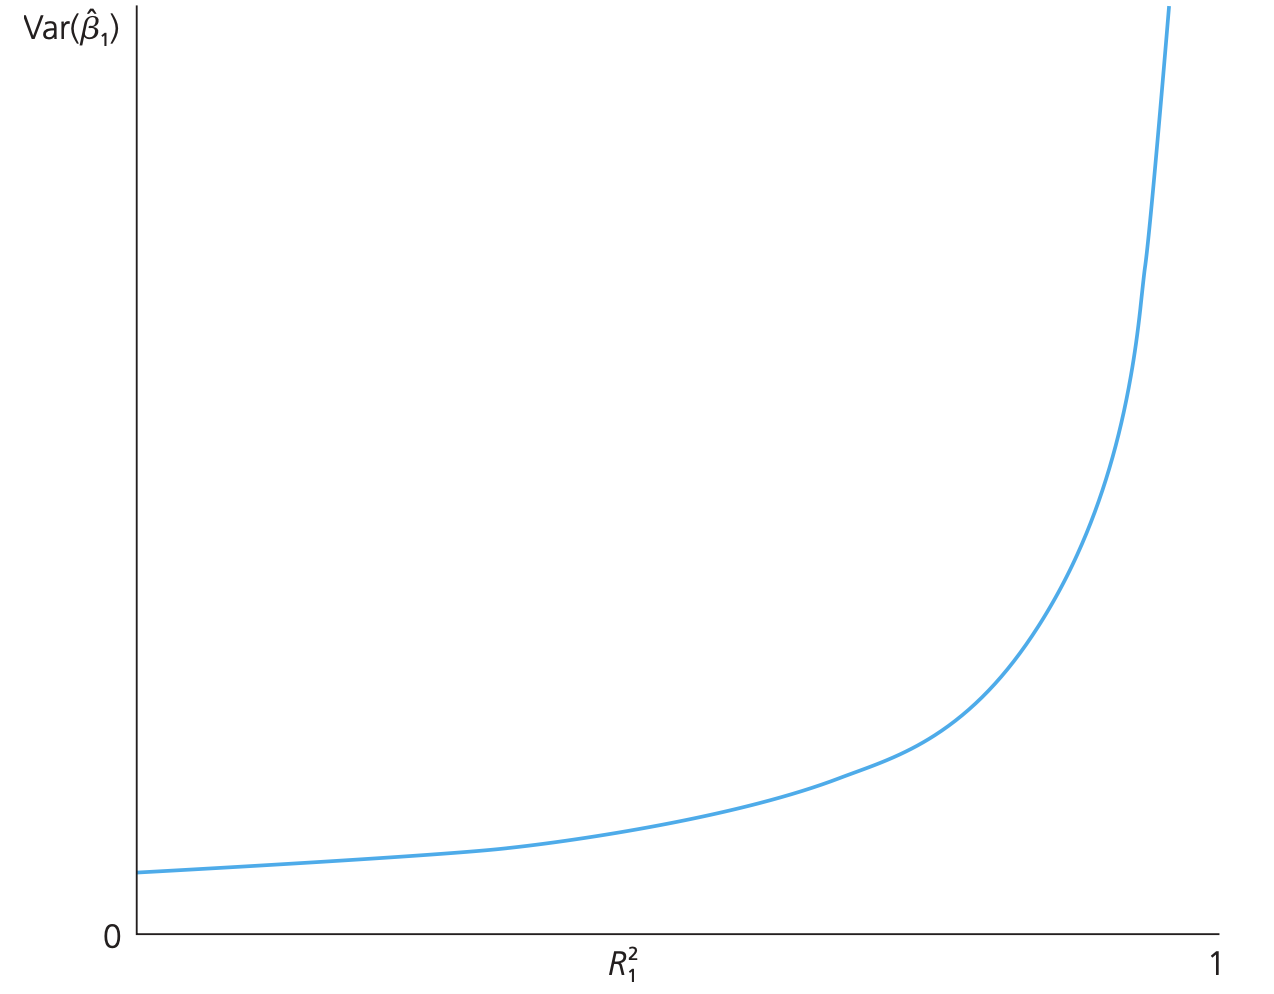
\includegraphics[width=0.5\textwidth]{figure3.1.png}
    \caption{Var($\hat{\beta_1}$) as a function of $R_1^2$.}
    \label{pic:p.90,fig3.1}
\end{figure}\\
A value of $R_1^2$ close to one indicates that $x_2$ explains much of the variation in $x_1$ in the sample. This means that $x_1$ and $x_2$ are highly correlated. As $R_1^2$ increases to one, Var($\hat{\beta_1}$) gets larger and larger. Thus, a high degree of linear relationship between $x_1$ and $x_2$ can lead to large variances for the OLS slope estimators. $R_1^2$ is the proportion of the total variation in $x_j$ that can be explained by the \textit{other} independent variables appearing in the equation.\\
One extreme case is when $R_j^2 = 0$ if and only if $x_j$ has zero sample correlation with \textit{every other} independent variable. The other extreme case is that $R_j^2 = 1$, is ruled out by Assumption MLR.3, because $R_j^2 = 1$ means that, in the sample , $x_j$ is a \textit{perfect} linear combination of some of the other independent variables in the regression. High(but not perfect) correlation between two or more independent variables is called \textbf{multicollinearity}.\\
One important thing to state is that: a case where $R_j^2$ is close to one is \textit{not} a violation of MLR.3.\\
Although the problem of multicollinearity cannot be clearly defined, one thing is clear: everything else being equal, for estimating $\beta_j$, it is better to have less correlation between $x_j$ and the other independent variables.
\begin{remark}
    \textbf{Variance inflation factor (VIF)}\\
    The VIF for slope coefficient $j$ is simply VIF$_j = 1/(1-R_j^2)$, precisely the term in $Var(\hat{\beta_j})$ that is determined by correlation between $x_j$ and other explanatory variables. We can write the $Var(\hat{\beta_j})$ in equation (\ref{eq:p.88,3.51}) as
    \begin{equation*}
        Var(\hat{\beta_j}) = \frac{\sigma^2}{SST_j} \cdot VIF_j,
    \end{equation*}
    which shows that VIF$_j$ is the factor by which $Var(\hat{\beta_j})$ is higher because $x_j$ is not uncorrelated with the other explanatory variables.\\
    Sometimes the value 10 is chosen: if VIF$_j$ is above 10  (equivalently, $R_j^2$ is above .9), then we conclude that multicollinearity is a ``problem'' for estimating $\beta_j$.
\end{remark}
\subsubsection{Variances in Misspecified Model}
Write the true population model, which satisfies the Gauss-Markov assumptions, as
\begin{equation*}
    y = \beta_0 + \beta_1x_1 + \beta_2x_2 + u.
\end{equation*}
We consider two estimators of $\beta_1$. The estimator $\hat{\beta_1}$ comes from the multiple regression
\begin{equation}
    \hat{y} = \hat{\beta_0} + \hat{\beta_1}x_1 + \hat{\beta_2}x_2. \label{eq:p.92,3.52}
\end{equation}
The estimator $\tilde{\beta_1}$ is obtained by omitting $x_2$ from the model and running a simple regression of $y$ on $x_1$: 
\begin{equation}
    \tilde{y} = \tilde{\beta_0} + \tilde{\beta_1}x_1 \label{eq:p.92,3.53}
\end{equation}
Now, we can write the variances for $\hat{\beta_1}$ and $\tilde{\beta_1}$:
\begin{align}
    Var(\hat{\beta_1}|x_1,x_2) &= \sigma^2 / \left[SST_1 (1 - R_1^2) \right]\label{eq:p.93,3.54} \\
    Var(\tilde{\beta_1}|x_1,x_2) &= \sigma^2 / SST_1 \label{eq:p.93,3.55}
\end{align}
Var($\tilde{\beta_1}$) is always \textit{smaller} than Var($\hat{\beta_1}$), unless $x_1$ and $x_2$ are uncorrelated in the sample, in which the two estimators $\hat{\beta_1}$ and $\tilde{\beta_1}$ are the same. Assuming that $x_1$ and $x_2$ are not uncorrelated, we can draw the following conclusions:
\begin{enumerate}
    \item When $\beta_2 \neq 0$, $\tilde{\beta_1}$ is biased, $\hat{\beta_1}$ is unbiased, and Var($\tilde{\beta_1}|x_1,x_2$) $<$ Var($\hat{\beta_1}|x_1,x_2$).
    \item When $\beta_2 = 0$, $\tilde{\beta_1}$ and $\hat{\beta_1}$ are both unbiased, and Var($\tilde{\beta_1}|x_1,x_2$) $<$ Var($\hat{\beta_1}|x_1,x_2$).
\end{enumerate}
One important thing is that any bias in $\tilde{\beta_1}$ does not shrink as the sample size grows.

\subsubsection{Estimating \texorpdfstring{$\sigma^2$}{sigma squared}: Standard Errors of the OLS Estimators}
The unbiased estimator of $\sigma^2$ in the general multiple regression case is 
\begin{equation}
    \hat{\sigma}^2 = (\sum_{i=1}^n \hat{u_i}^2) / (n-k-1) = \text{SSR} / (n-k-1) \label{eq:p.94,3.56}
\end{equation}
The term $n-k-1$ in (\ref{eq:p.94,3.56}) is the \textbf{degrees of freedom (\textit{df})} for the general OLS problem with $n$ observations and $k$ independent variables. $k+1$ parameters in a regression model with $k$ independent variables and an intercept.\\
The expected value of the sum of squared residuals is 
\begin{equation*}
    \mathbb{E}(\text{SSR}) = (n-k-1)\sigma^2.
\end{equation*}
Similarly to SLR, these can be written $\sum_{i=1}^{n} \hat{u_i} = 0$ and $\sum_{i=1}^{n} x_{ij}\hat{u_i} = 0$, where $j = 1, 2, \ldots, k$.
\begin{theorem}
    \textbf{Unbiased Estimation of $\sigma^2$}\\
    Under the Gauss-Markov assumptions MLR.1 through MLR.5, $\mathbb{E}(\hat{\sigma}^2) =  \mathbb{E}(\hat{\sigma}^2|\mathbf{x_1, \ldots, \mathbf{x_k}})=\sigma^2$
\end{theorem}
The positive square root of $\hat{\sigma}^2$, denoted $\hat{\sigma}$, is called the \textbf{standard error of the regression (SER)}.
\begin{remark}
    \textbf{Standard deviation of $\hat{\beta_j}$} which is just the square root of the variance:
    \begin{equation*}
        \text{sd}(\hat{\beta_j}) = \sigma/ \left[ \text{SST}_j(1-R_j^2)\right]^{1/2}.
    \end{equation*}
    Because $\sigma$ is unknown, we replace it with its estimator, $\hat{\sigma}$. This gives us the \textbf{standard error of} $\hat{\beta_j}$:
    \begin{equation}
        \text{se}(\hat{\beta_j}) = \hat{\sigma} \left[ \text{SST}_j(1-R_j^2)\right]^{1/2}.
        \label{eq:p.95,3.58}
    \end{equation}
    Because se($\hat{\beta_j}$) depends on $\hat{\sigma}$, the standard error has a sampling distribution. Also, the standard error formula in (\ref{eq:p.95,3.58}) is \textit{not} a valid estimator of sd($\hat{\beta_j}$) if the errors exhibit heteroskedasticity. 
\end{remark}

\subsection{Efficiency of OLS: The Gauss-Markov Theorem}
Under Assumptions MLR.1 through MLR.4, OLS is unbiased. While under Assumptions MLR.1 through MLR.5, the OLS estimator $\hat{\beta_j}$ for $\beta_j$ is the \textbf{best linear unbiased estimator (BLUE).} To introduce the theorem, we need to understand each component of the ``BLUE'':
\begin{enumerate}
    \item An unbiased estimator is: in the current context, an estimator, say, $\hat{\beta}_j$, of $\beta_j$ is an unbiased estimator of $\beta_j$ if $\mathbb{E}(\hat{\beta}_j) = \beta_j$ for any $\beta_0, \beta_1, \dots, \beta_k$.
    \item In the current context, an estimator $\hat{\beta}_j$ of $\beta_j$ is linear if, and only if, it can be expressed as a linear function of the data on the dependent variable:
    \begin{equation}
        \hat{\beta}_j = \sum_{i=1}^n w_{ij} y_i, \label{eq:p.95,3.60}
    \end{equation}
    where each $w_{ij}$ can be a function of the sample values of all the independent variables. The OLS estimators are linear, as can be seen from equation (\ref{eq:p.75,3.22}).
    \item For the current theorem, best is defined as \textit{having the smallest variance}.
\end{enumerate}
\begin{theorem}
    \textbf{Gauss-Markov Theorem}\\
    Let $\hat{\beta}_0, \hat{\beta}_1, \dots, \hat{\beta}_k$ denote the OLS estimators in model (\ref{eq:p.80,3.31}) under Assumptions MLR.1 through MLR.5. We have the following inequality:
    \begin{equation}
        \text{Var}(\hat{\beta}_j|x_1,\ldots, x_k) \leq \text{Var}(\tilde{\beta}_j|x_1,\ldots, x_),\ j = 0, 1, \ldots, k. 
    \end{equation}
    where $\forall \tilde{\beta_j} = \sum_{i=1}^n w_{ij}y_i$ and for each $\mathbb{E}(\tilde{\beta_j}) = \beta_j,\ j= 0, 1, \ldots, k$. (linear and unbiased)
\end{theorem}
The importance of the Gauss-Markov Theorem is that, when the standard set of assumptions
holds, we need not look for alternative unbiased estimators of the form in (\ref{eq:p.95,3.60}): none will be better than OLS.

\newpage

\section{Multiple Regression Analysis: Inference}
\setcounter{equation}{0}
\setcounter{theorem}{0}
\setcounter{assumption}{0}
This section will discuss some statistical inference: \textbf{Confidence Interval and Hypothesis test} \\
Sampling distribution of the OLS estimators
\begin{enumerate}
    \item [(i)] OLS estimators are r.v's.
    \item [(ii)] Mean and variance are known. 
    \item[(iii)] For C.I and Hypothesis tests additional assumption is needed. 
\end{enumerate}
\subsection{Sampling Distributions of the OLS Estimators}
\begin{assumption}
    \textbf{Normality of error terms (Assumption MLR.6)}\\
    The population error u is independent of the explanatory variables $x_1, x_2, \ldots, x_k$ and is normally distributed with zero mean and variance 
    $\sigma^2: u \overset{a}{\sim}\text{Normal}(0,\sigma^2)$.
\end{assumption}
Because $u$ is independent of the $x_j$ under MLR.6, $\mathbb{E}(u|x_1, \dots, x_k) = \mathbb{E}(u) = 0$ and $\text{Var}(u | x_1, \dots, x_k) = \text{Var}(u) = \sigma^2$. Thus, if we make Assumption MLR.6, then we are necessarily assuming MLR.4 and MLR.5.
\begin{remark} Some important facts:
    \begin{enumerate}
        \item Assumptions MLR.1 through MLR.6 are called the \textbf{classical linear model (CLM) assumptions}. It is best to think of the CLM assumptions as containing all of the Gauss-Markov assumptions \textit{plus} the assumption of a normally distributed error term.
        \item Under the CLM assumptions, the OLS estimators $\hat{\beta}_0, \hat{\beta}_1, \dots, \hat{\beta}_k$ are the \textbf{minimum variance unbiased estimators}, which means that OLS has the smallest variance among unbiased estimators; we no longer have to restrict our comparison to estimators that are linear in the $y_i$. \\
        $\Rightarrow$ OLS is the Best Unbiased Estimator.
        \item A succinct way to summarize the population assumptions of the CLM is
        \begin{equation*}
            y | \mathbf{x} \sim \text{Normal}(\beta_0 + \beta_1 x_1 + \beta_2 x_2 + \dots + \beta_k x_k, \sigma^2),
        \end{equation*}
        where $\mathbf{x}$ is again shorthand for $(x_1, \dots, x_k)$. Thus, conditional on $\mathbf{x}$, $y$ has a normal distribution with mean linear in $x_1, \dots, x_k$ and a constant variance.
        \item In any application, whether normality of $u$ can be assumed is really an empirical matter.
        \item Often, using a transformation, especially taking the log, yields a distribution that is closer to normal.
        \item At least, the error distribution should be \textit{close} to normal.
        \item Examples where normality cannot hold:
        \begin{itemize}
            \item wage (always positive)
            \item unemployment (only 0 or 1)
        \end{itemize}
        \item \textbf{Important}: For the purpose of statistical inference, nonnormality of the errors is not a serious problem with large sample sizes. (CLT)
    \end{enumerate}
\end{remark}
\begin{theorem}
    \textbf{Normal Sampling Distributions}\\
    Under the CLM assumptions MLR.1 through MLR.6, conditional on the sample values of the independent variables,
    \begin{equation}
        \hat{\beta}_j \sim \text{Normal}[\beta_j, \text{Var}(\hat{\beta}_j)], \label{eq:p.119,4.1}
    \end{equation}
    where $\text{Var}(\hat{\beta}_j)$ was given in Chapter 2 [equation (\ref{eq:p.88,3.51})]. Therefore,
    \begin{equation*}
        (\hat{\beta}_j - \beta_j)/\text{sd}(\hat{\beta}_j) \sim \text{Normal}(0, 1).
    \end{equation*}
\end{theorem}
Each $\hat{\beta}_j$ can be written as $\hat{\beta}_j = \beta_j + \sum_{i=1}^n w_{ij} u_i,$ where $w_{ij} = \hat{r}_{ij} / \text{SSR}_j$. Here, $\hat{r}_{ij}$ is the $i^{\text{th}}$ residual from the regression of the $x_j$ on all the other independent variables, and $\text{SSR}_j$ is the sum of squared residuals from this regression [see equation (\ref{eq:p.94,3.56})]. Because the $w_{ij}$ depend only on the independent variables, they can be treated as nonrandom. Thus, $\hat{\beta}_j$ is just a linear combination of the errors in the sample $\{u_i : i = 1, 2, \dots, n\}$. An important fact about independent normal random variables is that a linear combination of such random variables is normally distributed.\\
In addition to (\ref{eq:p.119,4.1}), any  linear combination of the $\hat{\beta}_0, \hat{\beta}_1, \ldots, \hat{\beta}_k$ is also normally distributed, and any subset of the $\hat{\beta}_j$ has a \textit{joint} normal distribution. \\
Before we move on to the Confidence Interval and Hypothesis test, we need the following result:
\begin{theorem}
    \textbf{$\mathbf{t}$ Distribution for the Standardized Estimators}\\
    Under the CLM assumptions MLR.1 through MLR.6,
    \begin{equation}
        (\hat{\beta}_j - \beta_j)/\text{se}(\hat{\beta}_j) \sim t_{n-k-1} = t_{\text{df}}, \label{eq:p.120,4.3}
    \end{equation}
    where $k + 1$ is the number of unknown parameters in the population model $y = \beta_0 + \beta_1 x_1 + \dots + \beta_k x_k + u$ ($k$ slope parameters and the intercept $\beta_0$) and $n - k - 1$ is the degrees of freedom (\textit{df}).
\end{theorem}
The $t$ distribution in (\ref{eq:p.120,4.3}) comes from the fact that the constant $\sigma$ in $\text{sd}(\hat{\beta}_j)$ has been replaced with the random variable $\hat{\sigma}$.
The proof shows that (\ref{eq:p.120,4.3}) can be written as the ratio of the standard normal random variable $(\hat{\beta}_j - \beta_j)/\text{sd}(\hat{\beta}_j)$ over the square root of $\hat{\sigma}^2 / \sigma^2$. These random variables can be shown to be independent, and $(n - k - 1)\hat{\sigma}^2 / \sigma^2 \sim \chi^2_{n-k-1}.$
\subsection{Confidence Intervals}
Construct a \textbf{confidence interval (CI)} for the population parameter $\beta_j$ and this is also called \textit{interval estimates}.\\
Using the fact that $(\hat{\beta}_j)-\beta_j/\text{se}(\hat{\beta}_j)$ has a $t$ distribution with $n - k - 1$ degrees of freedom [see (\ref{eq:p.120,4.3})], simple manipulation leads to a CI for the unknown $\beta_j$: a \textit{95\% confidence interval}, given by 
\begin{equation}
    \hat{\beta}_j \pm c \cdot \text{se}(\hat{\beta}_j), \label{eq:p.135,4.16}
\end{equation}
where the constant $c$ is the 97.5$^\text{th}$ percentile in a $t_{n-k-1}$ distribution.
The lower and upper bounds of the confidence interval are given by
\begin{equation*}
    \underline{\beta}_j \equiv \hat{\beta}_j - c \cdot \text{se}(\hat{\beta}_j)
\end{equation*}
and 
\begin{equation*}
    \overline{\beta}_j \equiv \hat{\beta}_j + c \cdot \text{se}(\hat{\beta}_j),
\end{equation*}
Three quantities are needed: $\hat{\beta}_j$, $\text{se}(\hat{\beta}_j)$, and $c$. The coefficient estimate and its standard error are reported by any regression package. To obtain the value $c$, we must know the degrees of freedom, $n - k - 1$, and the level of confidence—95\% in this case. Then, the value for $c$ is obtained from the $t_{n-k-1}$ distribution.\\
When $n - k - 1 > 120$, the $t_{n-k-1}$ distribution is close enough to normal to use the 97.5$^\text{th}$ percentile in a standard normal distribution for constructing a 95\% CI:
$\hat{\beta}_j \pm 1.96 \cdot \text{se}(\hat{\beta}_j).$\\
After a confidence interval is constructed, it is easy to carry out two-tailed hypothesis tests. If the null hypothesis is $H_0: \beta_j = a$, then $H_0$ is rejected against $H_1: \beta_j \neq a$ (at the 5\% significance level) if, and only if, $a$ is \textit{not} in the 95\% confidence interval.
\subsection{Testing Hypotheses about a Single Population Parameter: The t Test}
Theorem 2 is important in that it allows us to test hypotheses involving the $\beta_j$. We are interesting in testing the \textbf{null hypothesis}
\begin{equation}
    \text{H}_0 : \beta_j = 0, \label{eq:p.120,4.4}
\end{equation}
where $j$ corresponds to any of the $k$ independent variables. What (\ref{eq:p.120,4.4}) means is that $\beta_j$ measures the partial effect of $x_j$ on (the expected value of) $y$, after controlling for all other independent variables, (\ref{eq:p.120,4.4}) means that, once $x_1, x_2, \dots, x_{j-1}, x_{j+1}, \dots, x_k$ have been accounted for, $x_j$ has \textit{no effect} on the expected value of $y$.\\
The statistic we use to test (\ref{eq:p.120,4.4}) (against any alternative) is called \textit{“the” t statistic} or \textit{“the” t ratio} of $\hat{\beta}_j$ and is defined as
\begin{equation}
    t_{\hat{\beta}_j} \equiv \hat{\beta}_j / \text{se}(\hat{\beta}_j).
\end{equation}
The standard error of $\hat{\beta}_j$ is an estimate of the standard deviation of $\hat{\beta}_j$, in (\ref{eq:p.120,4.4}), $t_{\hat{\beta}_j}$ measures how many estimated standard deviations $\hat{\beta}_j$ is away from zero. This is precisely what we do in testing whether the mean of a population is zero, using the standard $t$ statistic from introductory statistics.\\
The distribution of test statistic under H$_0$:
\begin{equation*}
    t_{\hat{\beta}_j} \equiv \hat{\beta}_j / \text{se}(\hat{\beta}_j) = \text{(under H$_0$)} \frac{\hat{\beta}_j - \beta_j}{\text{se}(\hat{\beta}_j)} \sim t_{(n-k-1)}
\end{equation*}
Remember that we are testing hypotheses about the \textit{population} parameters. We are \textit{not} testing hypotheses about the estimates from a particular sample.
\subsubsection{Testing against One-Sided Alternatives}
Consider a \textbf{one-side alternative} of the form
\begin{equation}
    \text{H}_1 : \beta_j > 0 \label{eq:p.122,4.6}
\end{equation}
When we state the alternative as in equation (\ref{eq:p.122,4.6}), we are really saying that the null hypothesis is $H_0: \beta_j \leq 0$. How should we choose a rejection rule? We must first decide on a \textit{significance level} or the probability of rejecting $H_0$ when it is in fact true. \\
The \textbf{rejection rule} is that $H_0$ is rejected in favor of $H_1$ at the 5\% significance level if
\begin{equation}
    t_{\hat{\beta}_j} > c.\label{eq:p.122,4.7}
\end{equation}
As the degrees of freedom in the $t$ distribution get large, the $t$ distribution approaches the standard normal distribution. For example, when $n - k - 1 = 120$, the 5\% critical value for the one-sided alternative (\ref{eq:p.122,4.7}) is 1.658, compared with the standard normal value of 1.645. These are close enough for practical purposes; for degrees of freedom greater than 120, one can use the standard normal critical values.
\begin{figure}[h!]
    \centering
    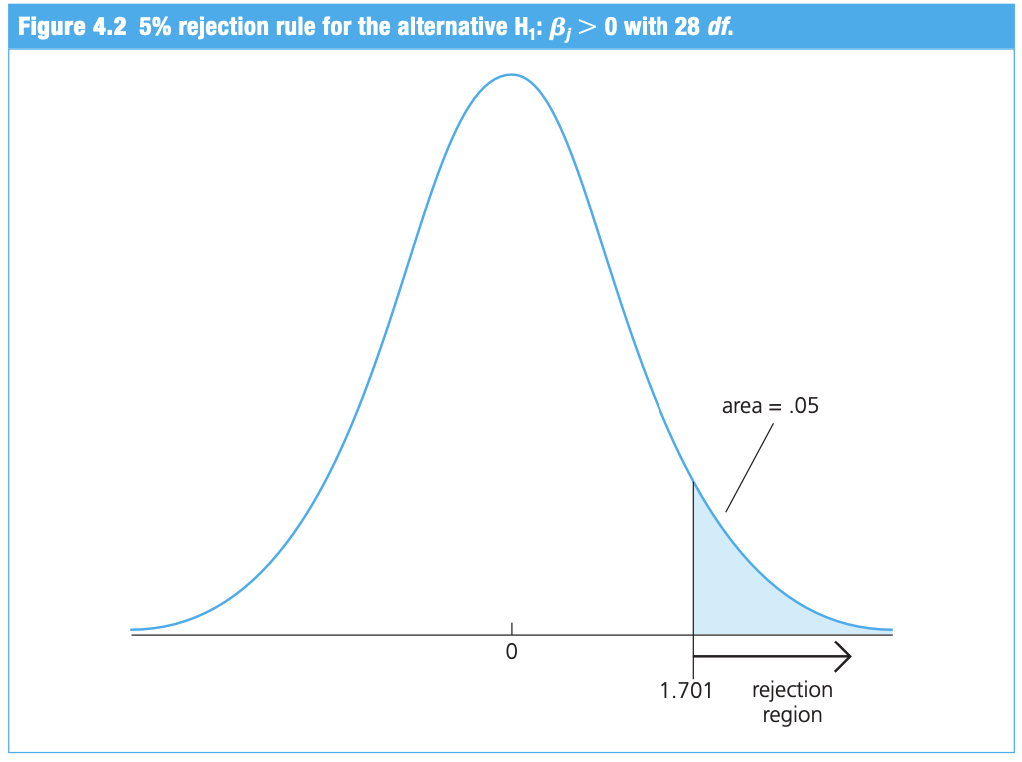
\includegraphics[width=0.5\textwidth]{figure4.2.png}
    \caption{example of rejection region}
    \label{pic:p.123,fig4.2}
\end{figure}\\
The one-sided alternative that the parameter is less than zero,
\begin{equation}
    H_1:\beta_j < 0 \label{eq:p.124,4.8}
\end{equation}
 In practice, it is easiest to think of the rejection rule as
\begin{equation}
    t_{\hat{\beta}_j} < -c. \label{eq:p.124,4.9}
\end{equation}
where $c$ is the critical value for the alternative $H1: \beta_j > 0$.\\
It is important to remember that, to reject $H_0$ against the negative alternative (\ref{eq:p.124,4.8}),we must get a negative $t$ statistic. A positive $t$ ratio, no matter how large, provides no evidence in favor of (\ref{eq:p.124,4.8}). 
\subsubsection{Two-Sided Alternatives}
It is common to test the null hypothesis $H_0:\beta_j = 0$ against a \textbf{two-sided alternative}; that is, 
\begin{equation}
    H_1 : \beta_j \neq 0 \label{eq:p.126,4.10}
\end{equation}
When the alternative is two-sided, we are interested in the \textit{absolute value} of the $t$ statistic. The rejection rule for $H_0: \beta_j = 0$ against (\ref{eq:p.126,4.10}) is
\begin{equation}
    |t_{\hat{\beta}_j}| > c,
\end{equation}
where $|\cdot|$ denotes absolute value and $c$ is an appropriately chosen critical value. To find $c$, we again specify a significance level, say 5\%. For a \textbf{two-tailed test}, $c$ is chosen to make the area in each tail of the $t$ distribution an equal 2.5\%.\\
If $H_0$ is rejected in favor of (\ref{eq:p.126,4.10}) at the 5\% level, we usually say that “$x_j$ is \textbf{statistically significant}, or statistically different from zero, at the 5\% level.” If $H_0$ is not rejected, we say that “$x_j$ is \textbf{statistically insignificant} at the 5\% level.”
\subsubsection{Testing Other Hypotheses about \texorpdfstring{$\beta_j$}{beta j}}
We sometimes want to test whether $\beta_j$ is equal to some other given constant. Two common examples are $\beta_j = 1$ and $\beta_j = -1$. Generally, if the null is stated as
\begin{equation}
    H_0: \beta_j = a_j, \label{eq:p.128,4.12}
\end{equation}
where $a_j$ is our hypothesized value of $\beta_j$, then the appropriate $t$ statistic is
\begin{equation*}
    t = (\hat{\beta}_j - a_j)/\text{se}(\hat{\beta}_j).
\end{equation*}
$t$ measures how many estimated standard deviations $\hat{\beta}_j$ is away from the hypothesized value of $\beta_j$. Then, $t$ statistic is written as
\begin{equation}
    t = \frac{(\textit{estimate} - \textit{hypothesized value})}{\textit{standard error}}. \label{eq:p.128,4.13}
\end{equation}
Under (\ref{eq:p.128,4.12}), this $t$ statistic is distributed as $t_{n-k-1}$ from Theorem 2.
\subsection{Testing Hypotheses about a Single Linear Combination of the Parameters}
We consider a model to compute the returns to education at junior colleges and four-year colleges and the model is
\begin{equation}
    \log(wage) = \beta_0 + \beta_1 jc + \beta_2 univ + \beta_3 exper + u, \label{eq:p.136,4.17}
\end{equation}
where
\begin{align*}
    jc & = \text{number of years attending a two-year college.} \\
    univ & = \text{number of years at a four-year college.} \\
    exper & = \text{months in the workforce.}
\end{align*}
The hypothesis of interest is whether one year at a junior college is worth one year at a university:
\begin{equation}
    H_0: \beta_1 = \beta_2. \label{eq:p.137,4.18}
\end{equation}
Under $H_0$, another year at a junior college and another year at a university lead to the same ceteris paribus percentage increase in \textit{wage}. The alternative of interest is one-sided: a year at a junior college is worth less than a year at a university.
\begin{equation}
    H_1: \beta_1 < \beta_2. \label{eq:p.137,4.19}
\end{equation}
We rewrite the null and alternative as $H_0: \beta_1 - \beta_2 = 0$ and $H_1: \beta_1 - \beta_2 < 0$, respectively.
The $t$ statistic is based on whether the estimated difference $\hat{\beta}_1 - \hat{\beta}_2$ is sufficiently less than zero to warrant rejecting (\ref{eq:p.137,4.18}) in favor of (\ref{eq:p.137,4.19}). Possible $t$ statistic is
\begin{equation}
    t = \frac{(\hat{\beta}_1 - \hat{\beta}_2)-(\beta_1-\beta_2)}{\text{se}(\hat{\beta}_1 - \hat{\beta}_2)}. \label{eq:p.137,4.20}
\end{equation}
To find $\text{se}(\hat{\beta}_1 - \hat{\beta}_2)$, we first obtain the variance of the difference.
\begin{equation}
    \text{Var}(\hat{\beta}_1 - \hat{\beta}_2) = \text{Var}(\hat{\beta}_1) + \text{Var}(\hat{\beta}_2) - 2\ \text{Cov}(\hat{\beta}_1, \hat{\beta}_2). \label{eq:p.137,4.22}
\end{equation}
The standard deviation of $\hat{\beta}_1 - \hat{\beta}_2$ is just the square root of (\ref{eq:p.137,4.22}), and, because $[\text{se}(\hat{\beta}_1)]^2$ is an unbiased estimator of $\text{Var}(\hat{\beta}_1)$, and similarly for $[\text{se}(\hat{\beta}_2)]^2$, we have
\begin{equation}
    \text{se}(\hat{\beta}_1 - \hat{\beta}_2) = \left\{ [\text{se}(\hat{\beta}_1)]^2 + [\text{se}(\hat{\beta}_2)]^2 - 2s_{12} \right\}^{1/2}, \label{eq:p.138,4.23}
\end{equation}
where $s_{12}$ denotes an estimate of $\text{Cov}(\hat{\beta}_1, \hat{\beta}_2)$.
Another way to test this model is much easier. Define a new parameter as the difference between $\beta_1$ and $\beta_2$: $\theta_1 = \beta_1 - \beta_2$. Then, we want to test
\begin{equation}
    H_0: \theta_1 = 0 \ \ \text{against} \ \ H_1: \theta_1 < 0. \label{eq:p.138,4.24}
\end{equation}
The $t$ statistic in (\ref{eq:p.137,4.20}) in terms of $\hat{\theta}_1$ is just $t = \hat{\theta}_1 / \text{se}(\hat{\theta}_1)$. Because $\theta_1 = \beta_1 - \beta_2$, we can also write $\beta_1 = \theta_1 + \beta_2$. Plugging this into (\ref{eq:p.136,4.17}) and rearranging gives the equation
\begin{align}
    \log(wage) &= \beta_0 + (\theta_1 + \beta_2)jc + \beta_2 univ + \beta_3 exper + u \notag \\
    &= \beta_0 + \theta_1 jc + \beta_2 (jc + univ) + \beta_3 exper + u. \label{eq:p.138,4.25}
\end{align}
If we want to directly estimate $\theta_1$ and obtain the standard error of $\hat{\theta}_1$, then we must construct the new variable $jc + univ$ and include it in the regression model in place of $univ$. So, define $totcoll = jc + univ$ and write (\ref{eq:p.138,4.25}) as
\begin{equation}
    \log(wage) = \beta_0 + \theta_1 jc + \beta_2 totcoll + \beta_3 exper + u. \label{eq:p.138,4.26}
\end{equation}
\subsection{Testing Multiple Linear Restrictions: The F Test}
\subsubsection{Testing Exclusion Restrictions}
Now, we want to test whether a \textit{group} of variables has no effect on the dependent
variable. We consider the he following model that explains major league baseball players' salaries:
\begin{equation}
    \log(salary) = \beta_0 + \beta_1 years + \beta_2 gamesyr + \beta_3 bavg + \beta_4 hrunsyr + \beta_5 rbisyr + u, \label{eq:p.139,4.28}
\end{equation}
where \textit{salary} is the 1993 total salary, \textit{years} is years in the league, \textit{gamesyr} is average games played per year, \textit{bavg} is career batting average (for example, $bavg = 250$), \textit{hrunsyr} is home runs per year, and \textit{rbisyr} is runs batted in per year.\\
In terms of the parameters of the model, the null hypothesis is stated as
\begin{equation}
    H_0: \beta_3 = 0, \ \beta_4 = 0, \ \beta_5 = 0. \label{eq:p.139,4.29}
\end{equation}
The null (4.29) constitutes three \textbf{exclusion restrictions}: if (4.29) is true, then \textit{bavg}, \textit{hrunsyr}, and \textit{rbisyr} have no effect on $\log(salary)$ after \textit{years} and \textit{gamesyr} have been controlled for and therefore should be excluded from the model. A test of multiple restrictions is called a \textbf{multiple hypotheses test} or a \textbf{joint hypotheses test}.\\
The appropriate alternative is simply
\begin{equation}
    H_1: H_0 \ \text{is not true}. \label{eq:p.139,4.30}
\end{equation}
The alternative (\ref{eq:p.139,4.30}) holds if at least one of $\beta_3$, $\beta_4$, or $\beta_5$ is different from zero. We must derive a test of multiple restrictions whose distribution is known and tabulated. \\
Because the OLS estimates are chosen to minimize the sum of squared residuals, the SSR \textit{always} increases when variables are dropped from the model. The question is whether this increase is large enough, \textit{relative} to the SSR in the model with all of the variables, to warrant rejecting the null hypothesis. We can have the without the three variables is simply
\begin{equation}
    \log(salary) = \beta_0 + \beta_1 years + \beta_2 gamesyr + u. \label{eq:p.140,4.32}
\end{equation}
Equation (\ref{eq:p.140,4.32}) is the \textbf{restricted model} for testing (\ref{eq:p.139,4.29}); model (\ref{eq:p.139,4.28}) is called the \textbf{unrestricted model}. The test statistic is:
\begin{equation*}
    F = \frac{(SSR_r - SSR_{ur})/3}{SSR_{ur}/(n-k-1)} \sim F_{3,(n-k-1)}
\end{equation*}
Write in a general case: the \textit{unrestricted model} with $k$ independent variables as
\begin{equation}
    y = \beta_0 + \beta_1 x_1 + \dots + \beta_k x_k + u; \label{eq:p.141,4.34}
\end{equation}
the number of parameters in the unrestricted model is $k + 1$. Suppose that we have $q$ exclusion restrictions to test: that is, the null hypothesis states that $q$ of the variables in (\ref{eq:p.141,4.34}) have zero coefficients. Assume that it is the last $q$ variables in the list of independent variables: $x_{k-q+1}, \dots, x_k$. The null hypothesis is stated as
\begin{equation}
    H_0: \beta_{k-q+1} = 0, \dots, \beta_k = 0, \label{eq:p.141,4.35}
\end{equation}
which puts $q$ exclusion restrictions on the model (\ref{eq:p.141,4.34}). When we impose the restrictions under $H_0$, we are left with the restricted model:
\begin{equation}
    y = \beta_0 + \beta_1 x_1 + \dots + \beta_{k-q} x_{k-q} + u. \label{eq:p.141,4.36}
\end{equation}
The \textbf{F statistic} (or \textbf{F ratio}) is defined by
\begin{equation}
    F \equiv \frac{(\text{SSR}_r - \text{SSR}_{ur}) / q}{\text{SSR}_{ur} / (n - k - 1)}, \label{eq:p.141,4.37}
\end{equation}
where $\text{SSR}_r$ is the sum of squared residuals from the restricted model and $\text{SSR}_{ur}$ is the sum of squared residuals from the unrestricted model.
Because $\text{SSR}_r$ can be no smaller than $\text{SSR}_{ur}$, the $F$ statistic is \textit{always} nonnegative (and almost always strictly positive).\\
The easiest way to remember where the SSRs appear is to think of $F$ as measuring the relative increase in SSR when moving from the unrestricted to the restricted model.\\
Basically, it can be shown that equation (\ref{eq:p.141,4.37}) is actually the ratio of two independent chi-square random variables, divided by their respective degrees of freedom. The numerator chi-square random variable has $q$ degrees of freedom, and the chi-square in the denominator has $n - k - 1$ degrees of freedom.\\
Let $c$ be the 95$^\text{th}$ percentile in the $F_{q, n-k-1}$ distribution. This critical value depends on $q$ (the numerator \textit{df}) and $n - k - 1$ (the denominator \textit{df}). Once $c$ has been obtained, we reject $H_0$ in favor of $H_1$ at the chosen significance level if
\begin{equation}
    F > c. \label{eq:p.142,4.40}
\end{equation}
If $H_0$ is rejected, then we say that $x_{k-q+1}, \dots, x_k$ are \textbf{jointly statistically significant} (or just \textit{jointly significant}) at the appropriate significance level. This test alone does not allow us to say which of the variables has a partial effect on $y$; they may all affect $y$ or maybe only one affects $y$. If the null is not rejected, then the variables are \textbf{jointly insignificant}, which often justifies dropping them from the model.
\subsubsection{The R-Squared Form of the F Statistic}
Using the fact that $\text{SSR}_r = \text{SST}(1 - R^2_r)$ and $\text{SSR}_{ur} = \text{SST}(1 - R^2_{ur})$, we can substitute into (\ref{eq:p.141,4.37}) to obtain
\begin{equation}
    F = \frac{(R^2_{ur} - R^2_r)/q}{(1 - R^2_{ur})/(n - k - 1)} = \frac{(R^2_{ur} - R^2_r)/q}{(1 - R^2_{ur})/df_{ur}}. \label{eq:p.145,4.41}
\end{equation}
(note that the SST terms cancel everywhere). This is called the \textbf{R-squared form of the F statistic}.
\subsubsection{The F Statistic for Overall Significance of a Regression}
In the model with $k$ independent variables, we can write the null hypothesis as
\begin{equation*}
    H_0: x_1, x_2, \dots, x_k \ \text{do not help to explain} \ y.    
\end{equation*}
It states that \textit{none} of the explanatory variables has an effect on $y$. The null is that all slope parameters are zero:
\begin{equation}
    H_0: \beta_1 = \beta_2 = \dots = \beta_k = 0, \label{eq:p.147,4.44}
\end{equation}
and the alternative is that at least one of the $\beta_j$ is different from zero. We can also state as $H_0: E(y|x_1, x_2, \dots, x_k) = E(y)$, so that knowing the values of $x_1, x_2, \dots, x_k$ does not affect the expected value of $y$.\\
There are $k$ restrictions in (4.44), and when we impose them, we get the restricted model
\begin{equation}
    y = \beta_0 + u; \label{eq:p.147,4.45}
\end{equation}
\textit{all} independent variables have been dropped from the equation. 
Therefore, the $F$ statistic for testing (\ref{eq:p.147,4.44}) can be written as
\begin{equation}
    \frac{R^2 / k}{(1 - R^2) / (n - k - 1)}, \label{eq:p.147,4.46}
\end{equation}
where $R^2$ is just the usual $R$-squared from the regression of $y$ on $x_1, x_2, \dots, x_k$.
The special form of (4.46) is valid only for testing joint exclusion of \textbf{all} independent variables. This is sometimes called determining the \textbf{overall significance of the regression}.\\
If we fail to reject (4.44), then there is no evidence that any of the independent variables help to explain $y$. 

\newpage

\section{Multiple Regression Analysis: OLS Asymptotics}
\setcounter{equation}{0}
\setcounter{theorem}{0}
\setcounter{assumption}{0}

Properties of OLS that hold for \textit{any} sample size:
\begin{itemize}
    \item Expected Values / Unbiasedness : MLR.1 -- MLR.4
    \item Variance formula : MLR.1 -- MLR.5
    \item Gauss-Markov Theorem : MLR.1 -- MLR.5
    \item Exact sampling distribution / tests : MLR.1 -- MLR.6
\end{itemize}
\subsection{Consistency}
Although not all useful estimators are unbiased, virtually all economists agree that \textbf{consistency} is a minimal requirement for an estimator. Let's review what  consistency is:
\begin{definition}
    \textbf{Consistency}\\
    An estimator $\hat{\theta_n}$ is \textit{consistent} for a parameter $\theta$ if 
    $$\mathbb{P}(\lvert\hat{\theta_n} - \theta \rvert < \epsilon) \rightarrow 1 $$ 
    for arbitrary $\epsilon > 0$ and $n\rightarrow \infty$. We will use the notation 
    $\hat{\theta_n} \xrightarrow{p} \theta$, i.e., convergence in probability
\end{definition}
An intuitive understanding, let $\hat{\beta_j}$ be the OLS estimator of $\beta_j$ for some $j$. For each $n$, $\hat{\beta_j}$ has a probability distribution. Because $\hat{\beta}_j$ is unbiased under Assumptions MLR.1 through MLR.4, this distribution has mean value $\beta_j$. If this estimator is consistent, then the distribution of $\hat{\beta}_j$ becomes more and more tightly distributed around $\beta_j$ as the sample size grows. As $n$ tends to infinity, the distribution of $\hat{\beta}_j$ collapses to the single point $\beta_j$. 
\begin{theorem}
    \textbf{Consistency of OLS}\\
    Under Assumptions MLR.1 through MLR.4, the OLS estimator 
    $\hat{\beta_{jn}} \xrightarrow{p} \beta_j,\ j=0, 1, \ldots, k$ (depend on $n$)
\end{theorem}
We can proof of this result is most easily developed using the matrix algebra methods, but 
prove this without difficulty in the case of the simple egression model. We write down the formula for $\hat{\beta_1}$, and then plug in $y_i = \beta_0 + \beta_1 x_{i1} + u_i$:
\begin{align}
    \hat{\beta}_1 &= \frac{\left( \sum_{i=1}^n (x_{i1} - \bar{x}_1) y_i \right)}
{\left( \sum_{i=1}^n (x_{i1} - \bar{x}_1)^2 \right)} \notag \\
&= \beta_1 + \frac{\left( n^{-1} \sum_{i=1}^n (x_{i1} - \bar{x}_1) u_i \right)}
{\left( n^{-1} \sum_{i=1}^n (x_{i1} - \bar{x}_1)^2 \right)} \notag \\
    &= \beta_1 + \frac{\left( n^{-1} \sum_{i=1}^n (x_{i1} - \bar{x}_1) (u_i - \bar{u}) \right)}{\left( n^{-1} \sum_{i=1}^n (x_{i1} - \bar{x}_1)^2 \right)} \label{eq:p.165,5.2} 
\end{align} 
here dividing both the numerator and denominator by $n$ does not change the expression
but allows us to directly apply the \textbf{law of large numbers}. By law of large numbers, 
averages in the second part of equation(\ref{eq:p.165,5.2}), we conclude that the numerator
and denominator converge in probability to the population quantities, $\text{Cov}(x_1, u)$ and $\text{Var}(x_1)$, respectively. Provided that $\text{Var}(x_1) \neq 0$—which is assumed in MLR.3—we can use the properties of \textit{probability limits} to get 
\begin{align}
    \text{plim} \hat{\beta}_1 &= \beta_1 + \frac{\text{Cov}(x_1, u)}{\text{Var}(x_1)} \notag\\
    &= \beta_1 \quad \text{because Cov}(x_1, u) = 0. \label{eq:p.165,5.3}
\end{align}                                                                                                                                                            
We have used the fact that $\mathbb{E}(u|x_1) = 0$ (Assumption MLR.4) implies 
that $x_1$ and $u$ are uncorrelated (have zero covariance).\\
The previous arguments, and equation (\ref{eq:p.165,5.3}) in particular, show that OLS is consistent in the simple regression case if we assume only zero correlation. This is also true in the general case. We now state this as an assumption.
\begin{assumption}
    \textbf{Zero Mean and Zero Correlation (Assumption MLR.4$'$)}\\
    $\mathbb{E}(u) = 0 \text{ and } Cov(x_i,u) = 0$ for $ j = 1, 2, \ldots, k $.
\end{assumption}
Assumption MLR.4$'$ is weaker than Assumption MLR.4 in the sense that the latter implies the former. The zero conditional mean assumption, $\mathbb{E}(u|x_1, \ldots, x_k) = 0$, is that \textit{any} function of the explanatory variables is uncorrelated with $u$. Assumption MLR.4$'$ requires only that each $x_j$ is uncorrelated with $u$ (and that $u$ has a zero mean in the population). There are two reasons that we still use Assumption MLR.4. First, OLS turns out to be biased (but consistent) under Assumption MLR.4$'$ if $\mathbb{E}(u \mid x_1, \ldots, x_k)$ depends on any of the $x_j$.\\
Second the zero conditional mean assumption means that we have properly modeled the population regression function (PRF). That is, under Assumption MLR.4 we can write
\begin{equation*}
    \mathbb{E}(y|x_1, \ldots, x_k) = \beta_0 + \beta_1 x_1 + \cdots + \beta_k x_k,
\end{equation*}
and so we can obtain partial effects of the explanatory variables on the average or expected value of $y$.\\
If we instead only assume Assumption MLR.4$'$, $\beta_0 + \beta_1 x_1 + \cdots + \beta_k x_k$ need not represent the PRF, and we face the possibility that some nonlinear functions of the $x_j$, such as $x_j^2$, could be correlated with the error $u$. 
\subsubsection{Deriving the Inconsistency in OLS}
\textit{Pending completion.}

\subsection{Asymptotic Normality and Large Sample Inference}
If the errors $u_1, u_2,\ldots , u_n$ are random draws from some distribution
other than the normal, the $\hat{\beta_j}$ will not be normally distributed, which means that the $t$ statistics will not have $t$ distributions and the $F$ statistics will not have $F$ distributions.\\
The normality plays no role in the unbiasedness of OLS, nor does it affect the conclusion that OLS is the best linear unbiased estimator under the Gauss-Markov assumptions. But exact inference based on t and F statistics requires MLR.6. We also need to know even though the $y_i$ are not from a normal distribution, we can use the \textbf{central limit theorem} to conclude that the OLS estimators satisfy \textbf{asymptotic normality}, which means they are approximately normally distributed in large enough sample sizes.
\begin{theorem}
    \textbf{Asymptotic Normality of OLS}\\
    Under the Gauss-Markov Assumptions MLR.1 through MLR.5,
    \begin{enumerate}
    \item[(i)] $\sqrt{n}(\hat{\beta}_j - \beta_j) \xrightarrow{a} \text{Normal}(0, \sigma^2 / a_j^2)$, where $\sigma^2 / a_j^2 > 0$ is the \textbf{asymptotic variance} of $\sqrt{n}(\hat{\beta}_j - \beta_j)$; or the slope coefficients, $a_j^2 = \text{plim}\left(n^{-1} \sum_{i=1}^n \hat{r}_{ij}^2 \right)$, where the $\hat{r}_{ij}$ are the residuals from regressing $x_j$ on the other independent variables. 
    We say that $\hat{\beta}_j$ is \textit{asymptotically normally distributed};
    \item[(ii)] $\hat{\sigma}^2$ is a consistent estimator of $\sigma^2 = \text{Var}(u)$,
    i.e., $\hat{\sigma}^2 \xrightarrow{p} \sigma^2$;
    \item[(iii)] For each $j$,
\begin{equation*}
    \frac{\hat{\beta}_j - \beta_j}{\text{sd}(\hat{\beta}_j)} \overset{a}{\sim} \text{Normal}(0, 1)
\end{equation*}
    and
\begin{equation}
        \frac{\hat{\beta}_j - \beta_j}{\text{se}(\hat{\beta}_j)} \overset{a}{\sim} \text{Normal}(0, 1), \ \text{(use CLT)} \label{eq:p.170,5.7}
\end{equation}
    where $\text{se}(\hat{\beta}_j)$ is the usual OLS standard error.
\end{enumerate}
\end{theorem}
Theorem 2 is useful because the normality Assumption MLR.6 has been dropped; the only
restriction on the distribution of the error is that it has finite variance, and we also assume zero conditional mean and homoskedasticity.\\
It is important to keep separate the notions of the population distribution of the error term, $u$, and the sampling distributions of the $\hat{\beta_j}$ as the sample size grows. Remember that the population distribution is immutable and has nothing to do with the sample size.\\
Theorem 2 says is that, regardless of the population distribution of $u$, the OLS estimators, when properly standardized, have approximate standard normal distributions. This approximation comes about by the central limit theorem because the OLS estimators involve the use of sample averages.\\
From an asymptotic point of view it does not matter that we have to replace $\sigma$ with $\hat{\sigma}$, replacing $\sigma$ with $\hat{\sigma}$ affects the exact distribution of the standardized $\hat{\beta_j}$. Under CLM assumptions, $(\hat{\beta_j} - \beta_j)/sd(\hat{\beta_j})$ has an exact Normal(0,1) distribution and   $(\hat{\beta_j} - \beta_j)/se(\hat{\beta_j})$ has an exact $t_{n-k-1}$ distribution.\\
How should we use the result in equation (\ref{eq:p.170,5.7})? From a practical perspective it is just as legitimate to write 
\begin{equation}
    \frac{\hat{\beta}_j - \beta_j}{\text{se}(\hat{\beta}_j)} \overset{a}{\sim} t_{n-k-1} = t_{\text{df}} \label{eq:p.171,5.8}
\end{equation}
because $t_{df}$ approaches the Normal(0,1) distribution as $df$ gets large. We know under the CLM assumptions the $t_{n-k-1}$ distribution holds exactly, it makes sense to treat
$(\hat{\beta_j} - \beta_j)/se(\hat{\beta_j})$ as a $t_{n-k-1}$ random variable generally, 
even when MLR.6 does not hold.\\
Depending on the distribution of $u$, more observations may be necessary before the \textbf{central limit theorem} delivers a useful approximation. Further, the quality of the approximation depends not just on n, but on the $df$, $n-k-1$: with more independent variables in the model, a larger sample size is usually needed to use the $t$ approximation.\\
It is very important to see that Theorem 2 \textit{does} require the homoskedasticity assumption (along with the zero conditional mean assumption). If Var$(y|x)$ is not constant, the usual $t$ statistics and confidence intervals are invalid no matter how large the sample size is; the central limit theorem does not bail us out when it comes to heteroskedasticity.\\
One conclusion of Theorem 2 is that $\hat{\sigma}^2$ is a consistent estimator of $\sigma^2$ and the consistency implies that $\hat{\sigma}$ is a consistent estimator of $\sigma$, which is important in establishing the asymptotic normality result in equation (\ref{eq:p.170,5.7}).
\begin{remark}
    \textbf{Asymptomatic Analysis of the OLS sampling error}\\
    The estimated variance of $\hat{\beta_j}$ is 
    \begin{equation}
        \widehat{\text{Var}(\hat{\beta}_j)} = \frac{\hat{\sigma}^2}{\text{SST}_j(1 - R_j^2)}, \label{eq:p.171,5.9}
    \end{equation}
    where SST$_j$ is the total sum of squares of $x_j$ in the sample, and $R_j^2$ is the R-squared from regressing $x_j$ on all of the other independent variables. As the sample size grows, $\hat{\sigma}^2$ converges in probability to the constant $\sigma^2$. Further, $R_j^2$ approaches a number strictly between zero and unity.\\
    The sample variance of $x_j$ is $\text{SST}_j / n$, and so $\text{SST}_j / n$ converges to $\text{Var}(x_j)$ as the sample size grows. This means that $\text{SST}_j$ grows at approximately the same rate as the sample size: $\text{SST}_j \approx n\sigma_j^2$, where $\sigma_j^2$ is the population variance of $x_j$. We find that $\widehat{\text{Var}(\hat{\beta}_j)}$ shrinks to zero at the rate of $1/n$; this is why larger sample sizes are better.\\
    Using the preceding argument, ewe can write 
    \begin{equation}
        \text{se}(\hat{\beta_j}) \approx c_j/\sqrt{n}. \label{eq:p.172,5.10}
    \end{equation}
    where $c_j$ is a positive constant that does \textit{not} depend on the sample size. The constant $c_j$ can be shown to be
    \begin{equation*}
        c_j = \frac{\sigma}{\sigma_j\sqrt{1-\rho_j^2}},
    \end{equation*}
    where $\sigma = \text{sd}(u)$, $\sigma_j = \text{sd}(x_j)$ and $\rho_j^2$ is the population $R$-squared from regressing $x_j$ on the other explanatory variables.\\
    Equation (\ref{eq:p.172,5.10}) is only the approximation but it is a useful rule of thumb: standard errors can be expected to shrink at a rate that is the inverse of the \textit{square root} of the sample size. (that is $1/\sqrt{n}$)
\end{remark}
\subsubsection{Other Large Sample Tests: The Lagrange Multiplier Statistic}
The form of the LM statistic we derive here relies on the Gauss-Markov assumptions, the same
assumptions that justify the F statistic in large samples. We do not need the normality assumption.\\
Consider the usual multiple regression model with $k$ independent variables:
\begin{equation}
    y = \beta_0 + \beta_1x_1 + \cdots + \beta_kx_k + u. \label{eq:p.172,5.11}
\end{equation}
We want to test last $q$ of these variables all have zero population parameters:
the null hypothesis is
\begin{equation}
    \text{H}_0: \beta_{k-q-1} = 0, \ldots, \beta_k = 0, \label{eq:p.173,5.12} 
\end{equation}
which puts $q$ exclusion restrictions on the model (\ref{eq:p.172,5.11}). As with F testing, the alternative to (\ref{eq:p.173,5.12}) is that at least one of the parameters is different from zero. The LM statistic requires estimation of the \textit{restricted} model only. \\
\paragraph{The Lagrange Multiplier Statistic for q Exclusion
Restrictions:}
\begin{enumerate}
    \item [(i)] Regress $y$ on the \textit{restricted} set of independent variables and save the residuals, $\tilde{u}$.
    \item[(ii)] Regress $u$ on all of the independent variables and obtain the $R$-squared, say, $R_u^2$. If $R_u^2$ is large which implies $\tilde{u}$ is explained by $x_{k-q-1}, \ldots, x_k$.
    \item[(iii)] Compute $LM = nR_u^2$ [the sample size times the $R$-squared obtained from step (ii)].
    \item[(iv)]  Compare $LM$ to the appropriate critical value, $c$, in a $\chi_q^2$ distribution if $LM > c$, the null hypothesis is rejected.  If not, we fail to reject H$_0$. The rejection rule is essentially the same as for $F$ testing.
\end{enumerate}

\newpage
 
\section{Multiple Regression Analysis: Further Issues}
\setcounter{equation}{0}
\setcounter{theorem}{0}
\setcounter{assumption}{0}
\subsection{Effects of Data Scaling on OLS Statistics}
\subsubsection{Beta Coefficients}
It is useful to obtain regression results when \textit{all} variables involved, the dependent as well as all the independent variables, have been \textit{standardized}. 
This means that we compute the \textit{z}-score for every variable in the sample. Then, we run a regression using the \textit{z}-scores. We start from the original OLS equation, with the variables in their original forms:
\begin{equation}
    y_i = \hat{\beta}_0 + \hat{\beta}_1 x_{i1} + \hat{\beta}_2 x_{i2} + \dots + \hat{\beta}_k x_{ik} + \hat{u}_i. \label{eq:p.184,6.2}
\end{equation}
If we average (\ref{eq:p.184,6.2}), use the fact that the $\hat{u}_i$ have a zero sample average, and subtract the result from (\ref{eq:p.184,6.2}), we get
\begin{equation*}
    y_i - \bar{y} = \hat{\beta}_1 (x_{i1} - \bar{x}_1) + \hat{\beta}_2 (x_{i2} - \bar{x}_2) + \dots + \hat{\beta}_k (x_{ik} - \bar{x}_k) + \hat{u}_i.
\end{equation*}
Let $\hat{\sigma}_y$ be the sample standard deviation for the dependent variable, let $\hat{\sigma}_1$ be the sample \textit{sd} for $x_1$, let $\hat{\sigma}_2$ be the sample \textit{sd} for $x_2$, and so on. Then, simple algebra gives the equation
\begin{equation}
    \frac{(y_i - \bar{y})}{\hat{\sigma}_y} = \left( \frac{\hat{\sigma}_1}{\hat{\sigma}_y} \right) \hat{\beta}_1 \left[ \frac{(x_{i1} - \bar{x}_1)}{\hat{\sigma}_1} \right] + \dots + \left( \frac{\hat{\sigma}_k}{\hat{\sigma}_y} \right) \hat{\beta}_k \left[ \frac{(x_{ik} - \bar{x}_k)}{\hat{\sigma}_k} \right] + \frac{\hat{u}_i}{\hat{\sigma}_y}.
    \label{eq:p.184,6.3}
\end{equation}
Each variable in (\ref{eq:p.184,6.3}) has been standardized by replacing it with its \textit{z}-score, and this has resulted in new slope coefficients. The slope coefficient on $(x_{i1} - \bar{x}_1)/\hat{\sigma}_1$ is $\left( \frac{\hat{\sigma}_1}{\hat{\sigma}_y} \right) \hat{\beta}_1$. Simply the original coefficient, $\hat{\beta}_1$, multiplied by the ratio of the standard deviation of $x_1$ to the standard deviation of $y$. The intercept has dropped out altogether.\\
Rewrite the (\ref{eq:p.184,6.3}), we have
\begin{equation}
    z_y = \hat{b}_1 z_1 + \hat{b}_2 z_2 + \dots + \hat{b}_k z_k + error, \label{eq:p.184,6.4}
\end{equation}
where $z_y$ denotes the \textit{z}-score of $y$, $z_1$ is the \textit{z}-score of $x_1$, and so on. The new coefficients are
\begin{equation}
    \hat{b}_j = \left( \frac{\hat{\sigma}_j}{\hat{\sigma}_y} \right) \hat{\beta}_j \ \text{for} \ j = 1, \dots, k. \label{eq:p.184,6.5}
\end{equation}
These $\hat{b}_j$ are traditionally called \textbf{beta coefficients}.\\ 
Beta coefficients receive their interesting meaning from equation (\ref{eq:p.184,6.4}): if $x_1$ increases by one standard deviation, then $\hat{y}$ changes by $\hat{b}_1$ standard deviations. It makes the scale of the regressors irrelevant, this equation puts the explanatory variables on equal footing.\\
When each $x_j$ has been standardized, comparing the magnitudes of the resulting beta coefficients is more compelling. When the regression equation has only a single explanatory variable, $x_1$, its standardized coefficient is simply the sample correlation coefficient between $y$ and $x_1$, which means it must lie in the range $-1$ to $1$.\\
To obtain the beta coefficients, we can always standardize $y$, $x_1, \dots, x_k$ and then run the OLS regression of the \textit{z}-score of $y$ on the \textit{z}-scores of $x_1, \dots, x_k$—where it is not necessary to include an intercept, as it will be zero. 

\subsection{More on Functional Form}
In this section, we will discuss some topics related to functional form: Logarithmic Functional Forms, Quadratics Form, Models with Interaction Terms and Average Partial Effects.

\subsubsection{More on Using Logarithmic Functional Forms}



\subsection{More on Goodness-of-Fit and Selection of Regressors}
Nothing about the classical linear model assumptions requires that $R^2$ be above any particular value; $R^2$ is simply an estimate of how much variation in $y$ is explained by $x1, x2,\ldots, x_k$ in the population.
\begin{itemize}
    \item High $R^2$ does \textbf{not} imply that there is a causal interpretation.
    \item Low $R^2$ does \textbf{not} preclude precise estimators of partial effects.
\end{itemize}
Remember, though, that the relative \textit{change} in the R-squared when variables are added to an equation is very useful: the $F$ statistic in (ch3 equation : \ref{eq:p.145,4.41}) for testing the joint significance crucially depends on the difference in $R$-squareds between the unrestricted and restricted models.

\subsubsection{Adjusted R-Squared}
It is usefully written $R$-squared as 
\begin{equation}
    R^2 = 1 - (SSR/n)/(SST/n). \label{eq:p.196,6.20}
\end{equation}
where SSR is the sum of squared residuals and SST is the total sum of squares. This expression reveals what $R^2$ is actually estimating. Define $\sigma_y^2$ as the population variance of $y$ and let $\sigma_u^2$ denote the population variance of the error term, $u$. The \textbf{population R-squared} is defined as
\begin{equation*}
    \rho^2 = 1 - \frac{\sigma_u^2}{\sigma_y^2};
\end{equation*}
this is the proportion of the variation in $y$ in the population explained by the independent variables.\\
$R^2$ estimates $\sigma_u^2$ by $\text{SSR}/n$, which we know to be biased. So why not replace $\text{SSR}/n$ with $\text{SSR}/(n - k - 1)$? Also, we can use $\text{SST}/(n - 1)$ in place of $\text{SST}/n$. Now, we arrive at the adjusted $R^2$:
\begin{align}
    \bar{R^2} &= 1 - \left[ \frac{\text{SSR}}{(n - k - 1)} \right] \Big/ \left[ \frac{\text{SST}}{(n - 1)} \right] \label{eq:p.196,6.21} \\
    &= 1 - \frac{\hat{\sigma}^2}{\text{SST}/(n - 1)} \\
    &= 1- \frac{\text{SSR}}{\text{SST}}\frac{(n-1)}{(n-k-1)}\\
    &= 1- (1-R^2)\frac{(n-1)}{(n-k-1)}.
\end{align}
because $\hat{\sigma}^2 = \text{SSR}/(n - k - 1)$.\\
$\bar{R^2}$ is \textit{not} generally known to be a better estimator. It is tempting to think that $\bar{R^2}$ corrects the bias in $R^2$ for estimating the population $R^2$, $\rho^2$, but it does not: the ratio of two unbiased estimators is not an unbiased estimator.\\
Using $\bar{R^2}$ has some attractiveness:
\begin{enumerate}
    \item $\bar{R^2}$ is that it imposes a penalty for adding additional independent variables to a model.
    \item $R^2$ can never fall when a new independent variable is added to a regression equation: this is because SSR never goes up (and usually falls) as more independent variables are added.
    \item If an independent variable is added to a regression, SSR falls, but so does the degrees of freedom in the regression, $n - k - 1$. The term $\text{SSR}/(n - k - 1)$ can go up or down when a new independent variable is added to a regression.
\end{enumerate}
If we add a new independent variable to a regression equation, $R^2$ increases if, and only if, the $t$ statistic on the new variable is greater than one in absolute value.



\newpage

\section{Heteroskedasticity}






\end{document}

